\documentclass[12pt,]{article}
\usepackage{lmodern}
\usepackage{amssymb,amsmath}
\usepackage{ifxetex,ifluatex}
\usepackage{fixltx2e} % provides \textsubscript
\ifnum 0\ifxetex 1\fi\ifluatex 1\fi=0 % if pdftex
  \usepackage[T1]{fontenc}
  \usepackage[utf8]{inputenc}
\else % if luatex or xelatex
  \ifxetex
    \usepackage{mathspec}
  \else
    \usepackage{fontspec}
  \fi
  \defaultfontfeatures{Ligatures=TeX,Scale=MatchLowercase}
    \setmainfont[]{TeX Gyre Pagella}
\fi
% use upquote if available, for straight quotes in verbatim environments
\IfFileExists{upquote.sty}{\usepackage{upquote}}{}
% use microtype if available
\IfFileExists{microtype.sty}{%
\usepackage{microtype}
\UseMicrotypeSet[protrusion]{basicmath} % disable protrusion for tt fonts
}{}
\usepackage[left=2.5cm,right=2.5cm,top=2.5cm,bottom=2.5cm]{geometry}
\usepackage{hyperref}
\hypersetup{unicode=true,
            pdftitle={Supplementary materials for: Modelling palaeoecological time series using generalized additive models},
            pdfauthor={Gavin L. Simpson},
            pdfkeywords={time series; generalized additive model; simultaneous interval; spline;
environmental change},
            pdfborder={0 0 0},
            breaklinks=true}
\urlstyle{same}  % don't use monospace font for urls
\usepackage{color}
\usepackage{fancyvrb}
\newcommand{\VerbBar}{|}
\newcommand{\VERB}{\Verb[commandchars=\\\{\}]}
\DefineVerbatimEnvironment{Highlighting}{Verbatim}{commandchars=\\\{\}}
% Add ',fontsize=\small' for more characters per line
\usepackage{framed}
\definecolor{shadecolor}{RGB}{248,248,248}
\newenvironment{Shaded}{\begin{snugshade}}{\end{snugshade}}
\newcommand{\KeywordTok}[1]{\textcolor[rgb]{0.13,0.29,0.53}{\textbf{{#1}}}}
\newcommand{\DataTypeTok}[1]{\textcolor[rgb]{0.13,0.29,0.53}{{#1}}}
\newcommand{\DecValTok}[1]{\textcolor[rgb]{0.00,0.00,0.81}{{#1}}}
\newcommand{\BaseNTok}[1]{\textcolor[rgb]{0.00,0.00,0.81}{{#1}}}
\newcommand{\FloatTok}[1]{\textcolor[rgb]{0.00,0.00,0.81}{{#1}}}
\newcommand{\ConstantTok}[1]{\textcolor[rgb]{0.00,0.00,0.00}{{#1}}}
\newcommand{\CharTok}[1]{\textcolor[rgb]{0.31,0.60,0.02}{{#1}}}
\newcommand{\SpecialCharTok}[1]{\textcolor[rgb]{0.00,0.00,0.00}{{#1}}}
\newcommand{\StringTok}[1]{\textcolor[rgb]{0.31,0.60,0.02}{{#1}}}
\newcommand{\VerbatimStringTok}[1]{\textcolor[rgb]{0.31,0.60,0.02}{{#1}}}
\newcommand{\SpecialStringTok}[1]{\textcolor[rgb]{0.31,0.60,0.02}{{#1}}}
\newcommand{\ImportTok}[1]{{#1}}
\newcommand{\CommentTok}[1]{\textcolor[rgb]{0.56,0.35,0.01}{\textit{{#1}}}}
\newcommand{\DocumentationTok}[1]{\textcolor[rgb]{0.56,0.35,0.01}{\textbf{\textit{{#1}}}}}
\newcommand{\AnnotationTok}[1]{\textcolor[rgb]{0.56,0.35,0.01}{\textbf{\textit{{#1}}}}}
\newcommand{\CommentVarTok}[1]{\textcolor[rgb]{0.56,0.35,0.01}{\textbf{\textit{{#1}}}}}
\newcommand{\OtherTok}[1]{\textcolor[rgb]{0.56,0.35,0.01}{{#1}}}
\newcommand{\FunctionTok}[1]{\textcolor[rgb]{0.00,0.00,0.00}{{#1}}}
\newcommand{\VariableTok}[1]{\textcolor[rgb]{0.00,0.00,0.00}{{#1}}}
\newcommand{\ControlFlowTok}[1]{\textcolor[rgb]{0.13,0.29,0.53}{\textbf{{#1}}}}
\newcommand{\OperatorTok}[1]{\textcolor[rgb]{0.81,0.36,0.00}{\textbf{{#1}}}}
\newcommand{\BuiltInTok}[1]{{#1}}
\newcommand{\ExtensionTok}[1]{{#1}}
\newcommand{\PreprocessorTok}[1]{\textcolor[rgb]{0.56,0.35,0.01}{\textit{{#1}}}}
\newcommand{\AttributeTok}[1]{\textcolor[rgb]{0.77,0.63,0.00}{{#1}}}
\newcommand{\RegionMarkerTok}[1]{{#1}}
\newcommand{\InformationTok}[1]{\textcolor[rgb]{0.56,0.35,0.01}{\textbf{\textit{{#1}}}}}
\newcommand{\WarningTok}[1]{\textcolor[rgb]{0.56,0.35,0.01}{\textbf{\textit{{#1}}}}}
\newcommand{\AlertTok}[1]{\textcolor[rgb]{0.94,0.16,0.16}{{#1}}}
\newcommand{\ErrorTok}[1]{\textcolor[rgb]{0.64,0.00,0.00}{\textbf{{#1}}}}
\newcommand{\NormalTok}[1]{{#1}}
\usepackage{graphicx,grffile}
\makeatletter
\def\maxwidth{\ifdim\Gin@nat@width>\linewidth\linewidth\else\Gin@nat@width\fi}
\def\maxheight{\ifdim\Gin@nat@height>\textheight\textheight\else\Gin@nat@height\fi}
\makeatother
% Scale images if necessary, so that they will not overflow the page
% margins by default, and it is still possible to overwrite the defaults
% using explicit options in \includegraphics[width, height, ...]{}
\setkeys{Gin}{width=\maxwidth,height=\maxheight,keepaspectratio}
\IfFileExists{parskip.sty}{%
\usepackage{parskip}
}{% else
\setlength{\parindent}{0pt}
\setlength{\parskip}{6pt plus 2pt minus 1pt}
}
\setlength{\emergencystretch}{3em}  % prevent overfull lines
\providecommand{\tightlist}{%
  \setlength{\itemsep}{0pt}\setlength{\parskip}{0pt}}
\setcounter{secnumdepth}{5}
% Redefines (sub)paragraphs to behave more like sections
\ifx\paragraph\undefined\else
\let\oldparagraph\paragraph
\renewcommand{\paragraph}[1]{\oldparagraph{#1}\mbox{}}
\fi
\ifx\subparagraph\undefined\else
\let\oldsubparagraph\subparagraph
\renewcommand{\subparagraph}[1]{\oldsubparagraph{#1}\mbox{}}
\fi

%%% Use protect on footnotes to avoid problems with footnotes in titles
\let\rmarkdownfootnote\footnote%
\def\footnote{\protect\rmarkdownfootnote}

%%% Change title format to be more compact
\usepackage{titling}

% Create subtitle command for use in maketitle
\newcommand{\subtitle}[1]{
  \posttitle{
    \begin{center}\large#1\end{center}
    }
}

\setlength{\droptitle}{-2em}

  \title{Supplementary materials for: Modelling palaeoecological time series
using generalized additive models}
    \pretitle{\vspace{\droptitle}\centering\huge}
  \posttitle{\par}
    \author{Gavin L. Simpson}
    \preauthor{\centering\large\emph}
  \postauthor{\par}
      \predate{\centering\large\emph}
  \postdate{\par}
    \date{August 16, 2018}

%\setromanfont{Constantia}
%\setromanfont{texgyrepagella.otf}
%\setmainfont{XITS}
%\setmathfont{XITS Math}
\setmathfont{TeX Gyre Pagella Math}
\setmathfont[range={\mathcal,\mathbfcal},StylisticSet=1]{XITS Math}

%\renewcommand\familydefault{\rmdefault} %comment to see the difference
%\DeclareMathAlphabet      {\mathup}{OT1}{\familydefault}{m}{n}

\newcommand{\uk}{\ensuremath{\mathit{U}^{\mathit{K}}_{\mathup{37}}}}

\newcommand{\loess}{\textsc{Loess}}

\usepackage{lineno}
\linenumbers

\begin{document}
\maketitle

\section{Introduction}\label{introduction}

This document is an annotated version of the R code used to fit the GAMs
and related analyses to the Small Water and Braya-Sø example data sets.

The following packages are required: \emph{mgcv}, \emph{scam},
\emph{ggplot2}, \emph{cowplot}, and \emph{tidyr}.

\begin{Shaded}
\begin{Highlighting}[]
\KeywordTok{library}\NormalTok{(}\StringTok{"mgcv"}\NormalTok{)}
\end{Highlighting}
\end{Shaded}

\begin{verbatim}
#> Loading required package: nlme
\end{verbatim}

\begin{verbatim}
#> This is mgcv 1.8-24. For overview type 'help("mgcv-package")'.
\end{verbatim}

\begin{Shaded}
\begin{Highlighting}[]
\KeywordTok{library}\NormalTok{(}\StringTok{"scam"}\NormalTok{)}
\end{Highlighting}
\end{Shaded}

\begin{verbatim}
#> This is scam 1.2-2.
\end{verbatim}

\begin{Shaded}
\begin{Highlighting}[]
\KeywordTok{library}\NormalTok{(}\StringTok{"ggplot2"}\NormalTok{)}
\KeywordTok{library}\NormalTok{(}\StringTok{"cowplot"}\NormalTok{)}
\end{Highlighting}
\end{Shaded}

\begin{verbatim}
#> 
#> Attaching package: 'cowplot'
\end{verbatim}

\begin{verbatim}
#> The following object is masked from 'package:ggplot2':
#> 
#>     ggsave
\end{verbatim}

\begin{Shaded}
\begin{Highlighting}[]
\KeywordTok{library}\NormalTok{(}\StringTok{"tidyr"}\NormalTok{)}
\end{Highlighting}
\end{Shaded}

In addition, the \emph{gratia} package is required; this in-development
package is not on CRAN but can be installed directly from GitHub using
functions from the \emph{devtools} package. To install the package,
install \emph{devtools} and then use
\texttt{devtools::install\_github()} to install \emph{gratia}, as shown
below:

\begin{Shaded}
\begin{Highlighting}[]
\NormalTok{## gratia is not on CRAN, install from github:}
\KeywordTok{install.packages}\NormalTok{(}\StringTok{"devtools"}\NormalTok{)}
\NormalTok{devtools::}\KeywordTok{install_github}\NormalTok{(}\StringTok{"gavinsimpson/gratia"}\NormalTok{)}
\end{Highlighting}
\end{Shaded}

Assuming that the installation of \emph{gratia} completes without error,
the package can be loaded as usual

\begin{Shaded}
\begin{Highlighting}[]
\KeywordTok{library}\NormalTok{(}\StringTok{"gratia"}\NormalTok{) }\CommentTok{# need to change the name of the package}
\end{Highlighting}
\end{Shaded}

The final environment-preparation step is to set the default
\emph{ggplot} theme, which the loading of \emph{cowplot} has
over-ridden. Here I use the more-minimal black-and-white theme
(\texttt{theme\_bw()})

\begin{Shaded}
\begin{Highlighting}[]
\NormalTok{## Default ggplot theme}
\KeywordTok{theme_set}\NormalTok{(}\KeywordTok{theme_bw}\NormalTok{())}
\end{Highlighting}
\end{Shaded}

\section{Load the data sets}\label{load-the-data-sets}

The example data sets are also stored on GitHub;
\url{https://github.com/gavinsimpson/frontiers-palaeo-additive-modelling}.
Once downloaded the data are read in and processed a little

\begin{Shaded}
\begin{Highlighting}[]
\NormalTok{## source Small Water data}
\NormalTok{small <-}\StringTok{ }\KeywordTok{readRDS}\NormalTok{(}\StringTok{"./data/small-water/small-water-isotope-data.rds"}\NormalTok{)}
\KeywordTok{head}\NormalTok{(small)}
\end{Highlighting}
\end{Shaded}

\begin{verbatim}
#>   Depth   d13C  TotalC d15N TotalN DryWeight     Year
#> 1   0.2 -27.57  806.49 3.05  64.21       8.2 2007.254
#> 2   0.4 -27.67  949.33 3.01  73.26       7.6 2006.510
#> 3   0.8 -27.63 1305.52 2.93  93.25      11.6 2004.941
#> 4   1.2 -27.62 1136.04 2.33  86.09       9.6 2003.269
#> 5   1.6 -27.48 1028.27 2.09  93.80      10.9 2001.496
#> 6   2.0 -27.39  809.91 2.66  79.98       9.9 1999.626
\end{verbatim}

\begin{Shaded}
\begin{Highlighting}[]
\NormalTok{## load braya so data set}
\NormalTok{braya <-}\StringTok{ }\KeywordTok{read.table}\NormalTok{(}\StringTok{"./data/braya-so/DAndrea.2011.Lake Braya So.txt"}\NormalTok{,}
                    \DataTypeTok{skip =} \DecValTok{84}\NormalTok{)}
\NormalTok{## clean up variable names}
\KeywordTok{names}\NormalTok{(braya) <-}\StringTok{ }\KeywordTok{c}\NormalTok{(}\StringTok{"Depth"}\NormalTok{, }\StringTok{"DepthUpper"}\NormalTok{, }\StringTok{"DepthLower"}\NormalTok{, }\StringTok{"Year"}\NormalTok{, }\StringTok{"YearYoung"}\NormalTok{,}
                  \StringTok{"YearOld"}\NormalTok{, }\StringTok{"UK37"}\NormalTok{)}
\NormalTok{## add a variable for the amount of time per sediment sample}
\NormalTok{braya <-}\StringTok{ }\KeywordTok{transform}\NormalTok{(braya, }\DataTypeTok{sampleInterval =} \NormalTok{YearYoung -}\StringTok{ }\NormalTok{YearOld)}
\KeywordTok{head}\NormalTok{(braya)}
\end{Highlighting}
\end{Shaded}

\begin{verbatim}
#>   Depth DepthUpper DepthLower     Year YearYoung YearOld   UK37
#> 1  0.25        0.0        0.5 1999.125   2006.00 1992.25 -0.640
#> 2  0.75        0.5        1.0 1985.375   1992.25 1978.50 -0.637
#> 3  1.25        1.0        1.5 1971.525   1978.50 1964.55 -0.614
#> 4  1.75        1.5        2.0 1957.575   1964.55 1950.60 -0.627
#> 5  2.25        2.0        2.5 1943.150   1950.60 1935.70 -0.633
#> 6  2.75        2.5        3.0 1928.250   1935.70 1920.80 -0.616
#>   sampleInterval
#> 1          13.75
#> 2          13.75
#> 3          13.95
#> 4          13.95
#> 5          14.90
#> 6          14.90
\end{verbatim}

\begin{Shaded}
\begin{Highlighting}[]
\NormalTok{## plot labels}
\NormalTok{d15n_label <-}\StringTok{ }\KeywordTok{expression}\NormalTok{(delta^\{}\DecValTok{15}\NormalTok{\}*N)}
\NormalTok{braya_ylabel <-}\StringTok{ }\KeywordTok{expression}\NormalTok{(}\KeywordTok{italic}\NormalTok{(U)[}\DecValTok{37}\NormalTok{]^\{}\KeywordTok{italic}\NormalTok{(k)\})}
\end{Highlighting}
\end{Shaded}

Plots of the two data sets are prepared using \emph{ggplot2}

\begin{Shaded}
\begin{Highlighting}[]
\NormalTok{## plot Small Water data}
\NormalTok{small_plt <-}\StringTok{ }\KeywordTok{ggplot}\NormalTok{(small, }\KeywordTok{aes}\NormalTok{(}\DataTypeTok{x =} \NormalTok{Year, }\DataTypeTok{y =} \NormalTok{d15N)) +}
\StringTok{    }\KeywordTok{geom_point}\NormalTok{() +}
\StringTok{    }\KeywordTok{labs}\NormalTok{(}\DataTypeTok{y =} \NormalTok{d15n_label, }\DataTypeTok{x =} \StringTok{"Year CE"}\NormalTok{)}

\NormalTok{## plot Braya-So data}
\NormalTok{braya_plt <-}\StringTok{ }\KeywordTok{ggplot}\NormalTok{(braya, }\KeywordTok{aes}\NormalTok{(}\DataTypeTok{x =} \NormalTok{Year, }\DataTypeTok{y =} \NormalTok{UK37)) +}
\StringTok{    }\KeywordTok{geom_line}\NormalTok{(}\DataTypeTok{colour =} \StringTok{"grey"}\NormalTok{) +}
\StringTok{    }\KeywordTok{geom_point}\NormalTok{() +}
\StringTok{    }\KeywordTok{labs}\NormalTok{(}\DataTypeTok{y =} \NormalTok{braya_ylabel, }\DataTypeTok{x =} \StringTok{"Year CE"}\NormalTok{)}

\NormalTok{## Recreate plot from manuscript}
\KeywordTok{plot_grid}\NormalTok{(small_plt, braya_plt, }\DataTypeTok{ncol =} \DecValTok{1}\NormalTok{, }\DataTypeTok{labels =} \StringTok{"auto"}\NormalTok{, }\DataTypeTok{align =} \StringTok{"hv"}\NormalTok{,}
          \DataTypeTok{axis =} \StringTok{"lr"}\NormalTok{)}
\end{Highlighting}
\end{Shaded}

\begin{center}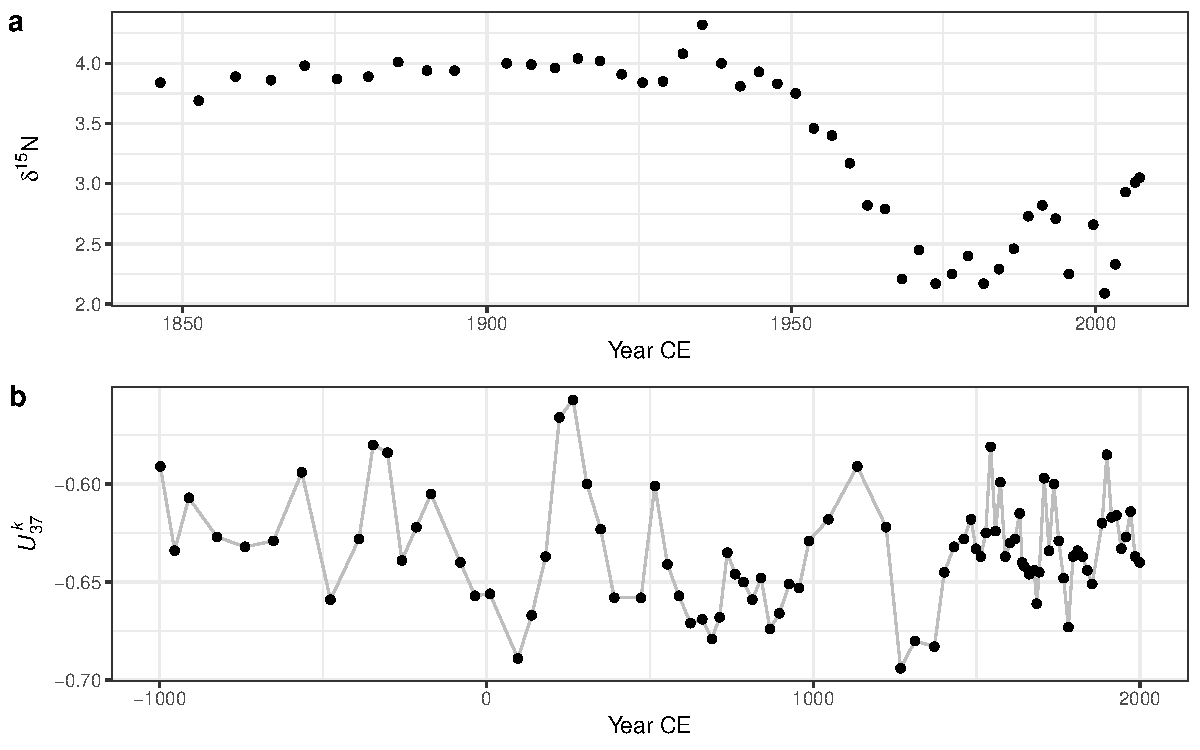
\includegraphics[width=0.8\linewidth]{supplementary-materials_files/figure-latex/data-figure-1} \end{center}

\section{Fitting GAMs}\label{fitting-gams}

Instead of following the structure of the paper exactly, the subsequent
sections focus on the two example data sets in turn, beginning with
Small Water.

\subsection{Small Water}\label{small-water}

A GAM is typically fitted using the \texttt{gam()} function from the
\emph{mgcv} package. The typical call includes a formula describing the
response variable and the linear predictor separated by the
\texttt{\textasciitilde{}} (tilde) symbol. The linear predictor part of
the model contains the smooth function of the time variable in the data
set, and is indicated using the \texttt{s()} function. Unless other
options are needed, we only need specify where the variables in the
formula can be found via the \texttt{data} argument, and that we wish to
use REML smoothness selection.

Putting this together we have the following function call to fit a
simple GAM to the Small Water isotope data

\begin{Shaded}
\begin{Highlighting}[]
\NormalTok{m <-}\StringTok{ }\KeywordTok{gam}\NormalTok{(d15N ~}\StringTok{ }\KeywordTok{s}\NormalTok{(Year, }\DataTypeTok{k =} \DecValTok{15}\NormalTok{), }\DataTypeTok{data =} \NormalTok{small, }\DataTypeTok{method =} \StringTok{"REML"}\NormalTok{)}
\end{Highlighting}
\end{Shaded}

As discussed in the paper, this model assumes that residuals\footnote{or
  equivalently that the observations, conditional upon the model, are
  independent.} are independent. To account for residual temporal
autocorrelation we can include a continuous-time first-order
autoregressive (CAR(1)) process in the model residuals for GAMs fitted
to data that are conditionally distributed Gaussian.

The GAM plus CAR(1) process is fitted to the Small Water data set using
the \texttt{gamm()} function. This fits GAMs as mixed effects models via
the \emph{nlme} package, which allows the use of correlation structures
in the model residuals via the \texttt{correlation} argument. Here, the
\texttt{corCAR1()} function is used to select the CAR(1) process and we
specify the ordering of samples via the \texttt{Year} variable in
\texttt{small}.

\begin{Shaded}
\begin{Highlighting}[]
\NormalTok{## fit small water GAM using gamm() with a CAR(1)}
\NormalTok{mod <-}\StringTok{ }\KeywordTok{gamm}\NormalTok{(d15N ~}\StringTok{ }\KeywordTok{s}\NormalTok{(Year, }\DataTypeTok{k =} \DecValTok{15}\NormalTok{), }\DataTypeTok{data =} \NormalTok{small,}
            \DataTypeTok{correlation =} \KeywordTok{corCAR1}\NormalTok{(}\DataTypeTok{form =} \NormalTok{~}\StringTok{ }\NormalTok{Year), }\DataTypeTok{method =} \StringTok{"REML"}\NormalTok{)}
\end{Highlighting}
\end{Shaded}

The estimated value of \(\phi\) for the CAR(1) can be extracted from the
fitted model via the \texttt{\$lme} component. Here we just extract the
correlation structure component.

\begin{Shaded}
\begin{Highlighting}[]
\NormalTok{## estimate of phi and confidence interval}
\NormalTok{smallPhi <-}\StringTok{ }\KeywordTok{intervals}\NormalTok{(mod$lme, }\DataTypeTok{which =} \StringTok{"var-cov"}\NormalTok{)$corStruct}
\NormalTok{smallPhi}
\end{Highlighting}
\end{Shaded}

\begin{verbatim}
#>        lower      est.     upper
#> Phi 0.282388 0.6026967 0.8539689
#> attr(,"label")
#> [1] "Correlation structure:"
\end{verbatim}

The object returned by \texttt{gamm()} includes both the linear mixed
model and GAM faces of the model, and as a result we need to access the
separate elements (\texttt{lme} and \texttt{gam} respectively) when
proceeding to explore the model fit. The model summary is prepared from
the \texttt{\$gam} component of the fitted model

\begin{Shaded}
\begin{Highlighting}[]
\NormalTok{## summary object}
\KeywordTok{summary}\NormalTok{(mod$gam)}
\end{Highlighting}
\end{Shaded}

\begin{verbatim}
#> 
#> Family: gaussian 
#> Link function: identity 
#> 
#> Formula:
#> d15N ~ s(Year, k = 15)
#> 
#> Parametric coefficients:
#>             Estimate Std. Error t value Pr(>|t|)    
#> (Intercept)  3.30909    0.03489   94.84   <2e-16 ***
#> ---
#> Signif. codes:  0 '***' 0.001 '**' 0.01 '*' 0.05 '.' 0.1 ' ' 1
#> 
#> Approximate significance of smooth terms:
#>           edf Ref.df     F p-value    
#> s(Year) 7.954  7.954 47.44  <2e-16 ***
#> ---
#> Signif. codes:  0 '***' 0.001 '**' 0.01 '*' 0.05 '.' 0.1 ' ' 1
#> 
#> R-sq.(adj) =  0.929   
#>   Scale est. = 0.037268  n = 48
\end{verbatim}

The output shows the estimated complexity of the fitted smooth,
expressed in terms of the effective degrees of freedom of the spline. An
associated \(F\) statistic and test of the null hypothesis of no trend
(effect) are also shown. Here the estimated trend provides strong
evidence against this null.

The CAR(1) process plotted in Figure 11 of the manuscript was prepared
using

\begin{Shaded}
\begin{Highlighting}[]
\NormalTok{## plot CAR(1) process}
\NormalTok{S <-}\StringTok{ }\KeywordTok{seq}\NormalTok{(}\DecValTok{0}\NormalTok{, }\DecValTok{50}\NormalTok{, }\DataTypeTok{length =} \DecValTok{100}\NormalTok{)}
\NormalTok{car1 <-}\StringTok{ }\KeywordTok{setNames}\NormalTok{(}\KeywordTok{as.data.frame}\NormalTok{(}\KeywordTok{t}\NormalTok{(}\KeywordTok{outer}\NormalTok{(smallPhi, S, }\DataTypeTok{FUN =} \StringTok{`}\DataTypeTok{^}\StringTok{`}\NormalTok{)[}\DecValTok{1}\NormalTok{, , ])),}
                 \KeywordTok{c}\NormalTok{(}\StringTok{"Lower"}\NormalTok{,}\StringTok{"Correlation"}\NormalTok{,}\StringTok{"Upper"}\NormalTok{))}
\NormalTok{car1 <-}\StringTok{ }\KeywordTok{transform}\NormalTok{(car1, }\DataTypeTok{S =} \NormalTok{S)}

\NormalTok{car1Plt <-}\StringTok{ }\KeywordTok{ggplot}\NormalTok{(car1, }\KeywordTok{aes}\NormalTok{(}\DataTypeTok{x =} \NormalTok{S, }\DataTypeTok{y =} \NormalTok{Correlation)) +}
\StringTok{    }\KeywordTok{geom_ribbon}\NormalTok{(}\KeywordTok{aes}\NormalTok{(}\DataTypeTok{ymax =} \NormalTok{Upper, }\DataTypeTok{ymin =} \NormalTok{Lower),}
                \DataTypeTok{fill =} \StringTok{"black"}\NormalTok{, }\DataTypeTok{alpha =} \FloatTok{0.2}\NormalTok{) +}
\StringTok{    }\KeywordTok{geom_line}\NormalTok{() +}
\StringTok{    }\KeywordTok{ylab}\NormalTok{(}\KeywordTok{expression}\NormalTok{(}\KeywordTok{italic}\NormalTok{(h) *}\StringTok{ }\NormalTok{(}\KeywordTok{list}\NormalTok{(Delta[t], varphi)))) +}
\StringTok{    }\KeywordTok{xlab}\NormalTok{(}\KeywordTok{expression}\NormalTok{(Delta[t] ~}\StringTok{ }\NormalTok{(years)))}
\NormalTok{car1Plt}
\end{Highlighting}
\end{Shaded}

\begin{center}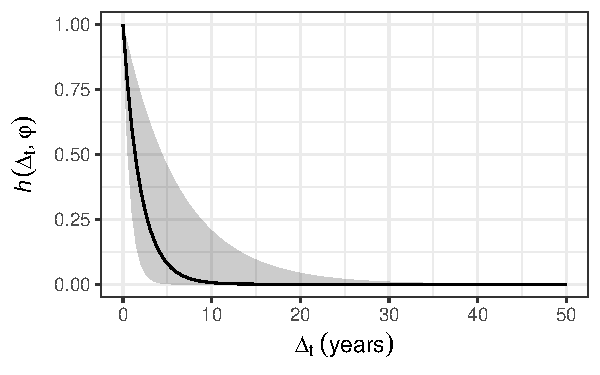
\includegraphics[width=0.8\linewidth]{supplementary-materials_files/figure-latex/car1-plot-1} \end{center}

The exponential decline in correlation with increasing separation is
evident here; once samples are \textasciitilde{}10 years apart, there is
little estimated dependence between them.

The next code chunk prepares a plot of the fitted GAMS. The general idea
is to predict from the fitted model for a fine grid of points over the
range of the time variable. Below I plot the trend for Small Water with
an approximate 95\% point-wise confidence interval that assumes
asymptotic normality

\begin{Shaded}
\begin{Highlighting}[]
\NormalTok{N <-}\StringTok{ }\DecValTok{300}   \CommentTok{# number of points at which to evaluate the smooth}

\NormalTok{## create new data to predict at; 200 evenly-spaced values over `Year`}
\NormalTok{newYear <-}\StringTok{ }\KeywordTok{with}\NormalTok{(small, }\KeywordTok{data.frame}\NormalTok{(}\DataTypeTok{Year =} \KeywordTok{seq}\NormalTok{(}\KeywordTok{min}\NormalTok{(Year), }\KeywordTok{max}\NormalTok{(Year),}
                                             \DataTypeTok{length.out =} \DecValTok{200}\NormalTok{)))}
\NormalTok{## Predict from the fitted model; note we predict from the $gam part}
\NormalTok{newYear <-}\StringTok{ }\KeywordTok{cbind}\NormalTok{(newYear,}
                 \KeywordTok{data.frame}\NormalTok{(}\KeywordTok{predict}\NormalTok{(mod$gam, newYear, }\DataTypeTok{se.fit =} \OtherTok{TRUE}\NormalTok{)))}
\NormalTok{## Create the confidence interval}
\NormalTok{crit.t <-}\StringTok{ }\KeywordTok{qt}\NormalTok{(}\FloatTok{0.975}\NormalTok{, }\DataTypeTok{df =} \KeywordTok{df.residual}\NormalTok{(mod$gam))}
\NormalTok{newYear <-}\StringTok{ }\KeywordTok{transform}\NormalTok{(newYear,}
                     \DataTypeTok{upper =} \NormalTok{fit +}\StringTok{ }\NormalTok{(crit.t *}\StringTok{ }\NormalTok{se.fit),}
                     \DataTypeTok{lower =} \NormalTok{fit -}\StringTok{ }\NormalTok{(crit.t *}\StringTok{ }\NormalTok{se.fit))}

\NormalTok{## Plot estimated trend}
\NormalTok{small_fitted <-}\StringTok{ }\KeywordTok{ggplot}\NormalTok{(newYear, }\KeywordTok{aes}\NormalTok{(}\DataTypeTok{x =} \NormalTok{Year, }\DataTypeTok{y =} \NormalTok{fit)) +}
\StringTok{    }\KeywordTok{geom_ribbon}\NormalTok{(}\KeywordTok{aes}\NormalTok{(}\DataTypeTok{ymin =} \NormalTok{lower, }\DataTypeTok{ymax =} \NormalTok{upper, }\DataTypeTok{x =} \NormalTok{Year), }\DataTypeTok{alpha =} \FloatTok{0.2}\NormalTok{,}
                \DataTypeTok{inherit.aes =} \OtherTok{FALSE}\NormalTok{, }\DataTypeTok{fill =} \StringTok{"black"}\NormalTok{) +}
\StringTok{    }\KeywordTok{geom_point}\NormalTok{(}\DataTypeTok{data =} \NormalTok{small, }\DataTypeTok{mapping =} \KeywordTok{aes}\NormalTok{(}\DataTypeTok{x =} \NormalTok{Year, }\DataTypeTok{y =} \NormalTok{d15N),}
               \DataTypeTok{inherit.aes =} \OtherTok{FALSE}\NormalTok{) +}
\StringTok{    }\KeywordTok{geom_line}\NormalTok{() +}
\StringTok{    }\KeywordTok{labs}\NormalTok{(}\DataTypeTok{y =} \NormalTok{d15n_label, }\DataTypeTok{x =} \StringTok{"Year CE"}\NormalTok{)}
\NormalTok{small_fitted}
\end{Highlighting}
\end{Shaded}

\begin{center}\includegraphics[width=0.8\linewidth]{supplementary-materials_files/figure-latex/small-plot-fitted-models-1} \end{center}

\subsection{Braya-Sø}\label{braya-s}

The same model as used for Small Water was also initially attempted with
the Braya-Sø data. However, in order to even fit the model with both a
smooth and the CAR(1) process, I had to change the default optimizer
used to estimate the model parameters, and reduce the basis dimension,
\texttt{k}, to a small number. I also fit the model using GCV, which is,
at the time of writing, the default in \texttt{gam()}, hence no
\texttt{method} argument

\begin{Shaded}
\begin{Highlighting}[]
\NormalTok{## fit the car(1) model --- needs optim as this is not a stable fit!}
\NormalTok{## also needs k setting lower than default}
\NormalTok{braya.car1 <-}\StringTok{ }\KeywordTok{gamm}\NormalTok{(UK37 ~}\StringTok{ }\KeywordTok{s}\NormalTok{(Year, }\DataTypeTok{k =} \DecValTok{5}\NormalTok{), }\DataTypeTok{data =} \NormalTok{braya, }
                   \DataTypeTok{correlation =} \KeywordTok{corCAR1}\NormalTok{(}\DataTypeTok{form =} \NormalTok{~}\StringTok{ }\NormalTok{Year),}
                   \DataTypeTok{method =} \StringTok{"REML"}\NormalTok{,}
                   \DataTypeTok{control =} \KeywordTok{list}\NormalTok{(}\DataTypeTok{niterEM =} \DecValTok{0}\NormalTok{, }\DataTypeTok{optimMethod =} \StringTok{"BFGS"}\NormalTok{, }
                                  \DataTypeTok{opt =} \StringTok{"optim"}\NormalTok{))}

\NormalTok{## fit model using GCV}
\NormalTok{braya.gcv <-}\StringTok{ }\KeywordTok{gam}\NormalTok{(UK37 ~}\StringTok{ }\KeywordTok{s}\NormalTok{(Year, }\DataTypeTok{k =} \DecValTok{30}\NormalTok{), }\DataTypeTok{data =} \NormalTok{braya)}

\NormalTok{## estimate of phi and confidence interval}
\NormalTok{brayaPhi <-}\StringTok{ }\KeywordTok{intervals}\NormalTok{(braya.car1$lme)$corStruct}
\NormalTok{brayaPhi}
\end{Highlighting}
\end{Shaded}

\begin{verbatim}
#>            lower      est. upper
#> Phi 2.680033e-31 0.2000156     1
#> attr(,"label")
#> [1] "Correlation structure:"
\end{verbatim}

Note the wide confidence interval --- effectively 0--1 --- on \(\phi\).
If you were to increase the value of \texttt{k} to be \texttt{k\ =\ 10}
in the \texttt{s(Year)} above, the model will fit but a warning message
will be emitted when trying to extract \(\phi\) due to a non-positive
definite model covariance matrix, indicating problems with the model.

To plot the GAMs fitted to the Braya-Sø time series, we repeat the
process used with the Small Water GAM, but we do this for both models
(GAMM + CAR(1) and GCV), using a critical value from the \(t\)
distribution to form the confidence interval

\begin{Shaded}
\begin{Highlighting}[]
\NormalTok{N <-}\StringTok{ }\DecValTok{300}   \CommentTok{# number of points at which to evaluate the smooth}

\NormalTok{## data to predict at}
\NormalTok{newBraya <-}\StringTok{ }\KeywordTok{with}\NormalTok{(braya, }\KeywordTok{data.frame}\NormalTok{(}\DataTypeTok{Year =} \KeywordTok{seq}\NormalTok{(}\KeywordTok{min}\NormalTok{(Year), }\KeywordTok{max}\NormalTok{(Year),}
                                              \DataTypeTok{length.out =} \NormalTok{N)))}
\NormalTok{## add predictions from GAMM + CAR(1) model}
\NormalTok{newBraya <-}\StringTok{ }\KeywordTok{cbind}\NormalTok{(newBraya,}
                  \KeywordTok{data.frame}\NormalTok{(}\KeywordTok{predict}\NormalTok{(braya.car1$gam, newBraya,}
                                     \DataTypeTok{se.fit =} \OtherTok{TRUE}\NormalTok{)))}
\NormalTok{crit.t <-}\StringTok{ }\KeywordTok{qt}\NormalTok{(}\FloatTok{0.975}\NormalTok{, }\DataTypeTok{df =} \KeywordTok{df.residual}\NormalTok{(braya.car1$gam))}
\NormalTok{newBraya <-}\StringTok{ }\KeywordTok{transform}\NormalTok{(newBraya,}
                      \DataTypeTok{upper =} \NormalTok{fit +}\StringTok{ }\NormalTok{(crit.t *}\StringTok{ }\NormalTok{se.fit),}
                      \DataTypeTok{lower =} \NormalTok{fit -}\StringTok{ }\NormalTok{(crit.t *}\StringTok{ }\NormalTok{se.fit))}

\NormalTok{## add GAM GCV results}
\NormalTok{fit_gcv <-}\StringTok{ }\KeywordTok{predict}\NormalTok{(braya.gcv, }\DataTypeTok{newdata =} \NormalTok{newBraya, }\DataTypeTok{se.fit =} \OtherTok{TRUE}\NormalTok{)}
\NormalTok{crit.t <-}\StringTok{ }\KeywordTok{qt}\NormalTok{(}\FloatTok{0.975}\NormalTok{, }\KeywordTok{df.residual}\NormalTok{(braya.gcv))}
\NormalTok{newGCV <-}\StringTok{ }\KeywordTok{data.frame}\NormalTok{(}\DataTypeTok{Year   =} \NormalTok{newBraya[[}\StringTok{"Year"}\NormalTok{]],}
                     \DataTypeTok{fit    =} \NormalTok{fit_gcv$fit,}
                     \DataTypeTok{se.fit =} \NormalTok{fit_gcv$se.fit)}
\NormalTok{newGCV <-}\StringTok{ }\KeywordTok{transform}\NormalTok{(newGCV,}
                    \DataTypeTok{upper =} \NormalTok{fit +}\StringTok{ }\NormalTok{(crit.t *}\StringTok{ }\NormalTok{se.fit),}
                    \DataTypeTok{lower =} \NormalTok{fit -}\StringTok{ }\NormalTok{(crit.t *}\StringTok{ }\NormalTok{se.fit))}
\NormalTok{newBraya <-}\StringTok{ }\KeywordTok{rbind}\NormalTok{(newBraya, newGCV)                }\CommentTok{# bind on GCV results}
\NormalTok{## Add indicator variable for model}
\NormalTok{newBraya <-}\StringTok{ }\KeywordTok{transform}\NormalTok{(newBraya,}
                      \DataTypeTok{Method =} \KeywordTok{rep}\NormalTok{(}\KeywordTok{c}\NormalTok{(}\StringTok{"GAMM (CAR(1))"}\NormalTok{, }\StringTok{"GAM (GCV)"}\NormalTok{), }
                                   \DataTypeTok{each =} \NormalTok{N))}

\NormalTok{## plot CAR(1) and GCV fits}
\NormalTok{braya_fitted <-}\StringTok{ }\KeywordTok{ggplot}\NormalTok{(braya, }\KeywordTok{aes}\NormalTok{(}\DataTypeTok{y =} \NormalTok{UK37, }\DataTypeTok{x =} \NormalTok{Year)) +}
\StringTok{    }\KeywordTok{geom_point}\NormalTok{() +}
\StringTok{    }\KeywordTok{geom_ribbon}\NormalTok{(}\DataTypeTok{data =} \NormalTok{newBraya,}
                \DataTypeTok{mapping =} \KeywordTok{aes}\NormalTok{(}\DataTypeTok{x =} \NormalTok{Year, }\DataTypeTok{ymax =} \NormalTok{upper, }\DataTypeTok{ymin =} \NormalTok{lower,}
                              \DataTypeTok{fill =} \NormalTok{Method),}
                \DataTypeTok{alpha =} \FloatTok{0.3}\NormalTok{, }\DataTypeTok{inherit.aes =} \OtherTok{FALSE}\NormalTok{) +}
\StringTok{    }\KeywordTok{geom_line}\NormalTok{(}\DataTypeTok{data =} \NormalTok{newBraya,}
              \DataTypeTok{mapping =} \KeywordTok{aes}\NormalTok{(}\DataTypeTok{y =} \NormalTok{fit, }\DataTypeTok{x =} \NormalTok{Year, }\DataTypeTok{colour =} \NormalTok{Method)) +}
\StringTok{    }\KeywordTok{labs}\NormalTok{(}\DataTypeTok{y =} \NormalTok{braya_ylabel, }\DataTypeTok{x =} \StringTok{"Year CE"}\NormalTok{) +}
\StringTok{    }\KeywordTok{scale_color_manual}\NormalTok{(}\DataTypeTok{values =} \KeywordTok{c}\NormalTok{(}\StringTok{"#5e3c99"}\NormalTok{, }\StringTok{"#e66101"}\NormalTok{)) +}
\StringTok{    }\KeywordTok{scale_fill_manual}\NormalTok{(}\DataTypeTok{values =} \KeywordTok{c}\NormalTok{(}\StringTok{"#5e3c99"}\NormalTok{, }\StringTok{"#e66101"}\NormalTok{)) +}
\StringTok{    }\KeywordTok{theme}\NormalTok{(}\DataTypeTok{legend.position =} \StringTok{"right"}\NormalTok{)}
\NormalTok{braya_fitted}
\end{Highlighting}
\end{Shaded}

\begin{center}\includegraphics[width=0.8\linewidth]{supplementary-materials_files/figure-latex/braya-plot-fitted-models-1} \end{center}

Figure 6 in the manuscript was produced using:

\begin{Shaded}
\begin{Highlighting}[]
\KeywordTok{plot_grid}\NormalTok{(small_fitted, braya_fitted, }\DataTypeTok{ncol =} \DecValTok{1}\NormalTok{, }\DataTypeTok{labels =} \StringTok{"auto"}\NormalTok{,}
          \DataTypeTok{align =} \StringTok{"hv"}\NormalTok{, }\DataTypeTok{axis =} \StringTok{"lr"}\NormalTok{)}
\end{Highlighting}
\end{Shaded}

\subsubsection{Checking if the size of the basis expansion is
sufficient}\label{checking-if-the-size-of-the-basis-expansion-is-sufficient}

For the Braya-Sø data, clearly we are not able to identify both the
wiggly trend and the CAR(1) process in a single model. We proceed by
fitting a simple GAM via \texttt{gam()} with REML smoothness selection
and a moderate number of basis functions --- here we set
\texttt{k\ =\ 15} for illustration.

\begin{Shaded}
\begin{Highlighting}[]
\NormalTok{braya_low_k <-}\StringTok{ }\KeywordTok{gam}\NormalTok{(UK37 ~}\StringTok{ }\KeywordTok{s}\NormalTok{(Year, }\DataTypeTok{k =} \DecValTok{15}\NormalTok{), }\DataTypeTok{data =} \NormalTok{braya, }\DataTypeTok{method =} \StringTok{"REML"}\NormalTok{)}
\end{Highlighting}
\end{Shaded}

Before proceeding, we should perform a check to determine if the number
of basis functions requested is sufficient to capture the wiggliness in
the data. This test is provided by \texttt{gam.check()}

\begin{Shaded}
\begin{Highlighting}[]
\KeywordTok{gam.check}\NormalTok{(braya_low_k)}
\end{Highlighting}
\end{Shaded}

\begin{verbatim}
#> 
#> Method: REML   Optimizer: outer newton
#> full convergence after 6 iterations.
#> Gradient range [-4.468978e-08,8.696768e-10]
#> (score -187.2524 & scale 0.000689802).
#> Hessian positive definite, eigenvalue range [0.5525272,43.5153].
#> Model rank =  15 / 15 
#> 
#> Basis dimension (k) checking results. Low p-value (k-index<1) may
#> indicate that k is too low, especially if edf is close to k'.
#> 
#>            k'   edf k-index p-value    
#> s(Year) 14.00  2.62    0.56  <2e-16 ***
#> ---
#> Signif. codes:  0 '***' 0.001 '**' 0.01 '*' 0.05 '.' 0.1 ' ' 1
\end{verbatim}

The first few lines of output from \texttt{gam.check()} include
information on the model fit, whether the algorithm converged, and some
diagnostics from the optimization at convergence --- you are unlikely to
need this information, but it can be useful in diagnosing problems with
model fitting or when reporting problems to Simon Wood, the developer of
the \emph{mgcv} package. In the table at the bottom of the output from
\texttt{gam.check()}, the column labelled \texttt{k\textquotesingle{}}
is the size of the basis used to fit the model (the number of basis
functions). Note that the stated value is 14 and not the requested 15
functions because the constant basis function has been removed due to it
being confounded with the model constant term, the intercept. The column
labelled \texttt{edf} indicates the \emph{effective degrees of freedom}
for the estimated smooth, which is a measure of the complexity or
wiggliness of the final smooth. The \texttt{k-index} column contains the
value of a test statistic for a test of a sufficient number of basis
functions --- ideally, we'd like the value of \texttt{k-index} to be
close to or greater than 1. The quoted \emph{p} value measures the
support for the null hypothesis that enough basis functions were
available. In practial terms, the low \texttt{k-index} and very low
\emph{p} value shown above strongly suggest that the requested number of
basis functions used to fit the model was too low.

The solution is to increase \texttt{k}, say by doubling the original
value, and refit the model and perform the basis dimension check using
\texttt{gam.check()}, repeating this process until \texttt{k-index} is
close to or greater than 1 and the \emph{p} value is larger than a
desired threshold. In my experience fitting GAMs to palaeoenvironmental
time series, it may not be possible with some data sets to increase
\texttt{k} large enough to result in a \texttt{k-index} \textgreater{} 1
and a \emph{p} value \textgreater{} 0.05, given the available number of
samples. It is important to remember that the test provided by
\texttt{gam.check()} is only an heuristic one and shouldn't be seen as
infallible. If you find yourself increasing \texttt{k} to large values
relative to the number of samples in your data set without achieving a
\texttt{k-index} \textgreater{} 1 or \emph{p} \textgreater{} 0.05, then
note the value in the \texttt{edf} column as you increase \texttt{k}. If
the \texttt{edf} of the model changes little as you continue to increase
\texttt{k}, this may be evidence that the test is failing in this
particular instance and that the estimated smooth is not dependent on
the value of \texttt{k} chosen.

\subsection{Accounting for heteroscedasticity due to time
averaging}\label{accounting-for-heteroscedasticity-due-to-time-averaging}

To proceed with the Braya-Sø example, we need to increase the basis
dimension, fit using \texttt{method\ =\ "REML"}. As discussed in the
manuscript, we should also account for the non-constant variance, or
\emph{heteroscedasticity}, that may arise due to variation in the amount
of time (or ``lake years'') that each sample represents. All else equal,
we expect that samples that average more time have lower variance than
those that average a smaller amount of time. To include information
about the expected heteroscedasticity in the GAM we can use
observational weights\footnote{This simple solution is for a Gaussian
  GAM. For models with other distributions, the exact interpretation of
  observational weights will vary. For such data, where the conditional
  mean and variance of the observations are linked, the use of
  location-scale, or distributional, models may be more apporpriate and
  informative.}. Here, I use the \texttt{sampleInterval} variable that I
created earlier as the measure of lake years per sample, and, to avoid
changing the model likelihood, the weights use are the values of
\texttt{sampleInterval} divided by the mean of \texttt{sampleInterval}:

\begin{Shaded}
\begin{Highlighting}[]
\NormalTok{braya_reml <-}\StringTok{ }\KeywordTok{gam}\NormalTok{(UK37 ~}\StringTok{ }\KeywordTok{s}\NormalTok{(Year, }\DataTypeTok{k =} \DecValTok{40}\NormalTok{), }\DataTypeTok{data =} \NormalTok{braya,}
                  \DataTypeTok{method =} \StringTok{"REML"}\NormalTok{,}
                  \DataTypeTok{weights =} \NormalTok{sampleInterval /}\StringTok{ }\KeywordTok{mean}\NormalTok{(sampleInterval))}
\KeywordTok{summary}\NormalTok{(braya_reml)}
\end{Highlighting}
\end{Shaded}

\begin{verbatim}
#> 
#> Family: gaussian 
#> Link function: identity 
#> 
#> Formula:
#> UK37 ~ s(Year, k = 40)
#> 
#> Parametric coefficients:
#>              Estimate Std. Error t value Pr(>|t|)    
#> (Intercept) -0.633741   0.001929  -328.5   <2e-16 ***
#> ---
#> Signif. codes:  0 '***' 0.001 '**' 0.01 '*' 0.05 '.' 0.1 ' ' 1
#> 
#> Approximate significance of smooth terms:
#>           edf Ref.df     F p-value    
#> s(Year) 27.45  32.36 7.782  <2e-16 ***
#> ---
#> Signif. codes:  0 '***' 0.001 '**' 0.01 '*' 0.05 '.' 0.1 ' ' 1
#> 
#> R-sq.(adj) =  0.744   Deviance explained = 82.4%
#> -REML = -175.61  Scale est. = 0.00024757  n = 89
\end{verbatim}

If we now check if 39 (\texttt{k\ =\ 40}) basis functions is sufficient

\begin{Shaded}
\begin{Highlighting}[]
\KeywordTok{gam.check}\NormalTok{(braya_reml)}
\end{Highlighting}
\end{Shaded}

\begin{verbatim}
#> 
#> Method: REML   Optimizer: outer newton
#> full convergence after 9 iterations.
#> Gradient range [-1.105422e-06,1.500959e-07]
#> (score -175.6093 & scale 0.0002475669).
#> Hessian positive definite, eigenvalue range [2.644434,47.78257].
#> Model rank =  40 / 40 
#> 
#> Basis dimension (k) checking results. Low p-value (k-index<1) may
#> indicate that k is too low, especially if edf is close to k'.
#> 
#>           k'  edf k-index p-value
#> s(Year) 39.0 27.5    1.27    0.99
\end{verbatim}

we note that the value of \texttt{k-index} is now greater than 1 and the
\emph{p} value suggests there is very little evidence against the null
hypothesis. This result strongly suggests that there were sufficient
basis functions used to estimated the trend.

Also note that the \texttt{edf} of the estimated smooth is considerably
below the maximum (\texttt{k\textquotesingle{}}). This is the effect of
the smoothness penalty removing the excessive wiggliness possible with
39 basis functions. If the \texttt{edf} were close to
\texttt{k\textquotesingle{}}, you might consider increasing \texttt{k}
by a modest amount (in this instance by 5 or 10 additional basis
functions) to assure yourself that you have sufficient basis functions.
This has the additional advantage of allowing a richer set of smooths of
a given complexity (\texttt{edf}) to be represented using this larger
set of basis functions, which may improve the model fit to the data
without changing the \texttt{edf} too much.

\section{Posterior simulation}\label{posterior-simulation}

Samples from the posterior distribution of a GAM can be drawn using the
\texttt{simulate()} methods from the \emph{gratia} package.

\begin{Shaded}
\begin{Highlighting}[]
\KeywordTok{set.seed}\NormalTok{(}\DecValTok{1}\NormalTok{) }\CommentTok{# set the random seed to make this reproducible}
\NormalTok{nsim <-}\StringTok{ }\DecValTok{20}  \CommentTok{# how many simulations to draw}

\NormalTok{## do the simulations}
\NormalTok{sims <-}\StringTok{ }\KeywordTok{simulate}\NormalTok{(mod, }\DataTypeTok{nsim =} \NormalTok{nsim, }\DataTypeTok{newdata =} \NormalTok{newYear, }\DataTypeTok{unconditional =} \OtherTok{TRUE}\NormalTok{)}

\NormalTok{## rearrange the output into a long/tidy format}
\KeywordTok{colnames}\NormalTok{(sims) <-}\StringTok{ }\KeywordTok{paste0}\NormalTok{(}\StringTok{"sim"}\NormalTok{, }\KeywordTok{seq_len}\NormalTok{(nsim))}
\NormalTok{sims <-}\StringTok{ }\KeywordTok{setNames}\NormalTok{(}\KeywordTok{stack}\NormalTok{(}\KeywordTok{as.data.frame}\NormalTok{(sims)), }\KeywordTok{c}\NormalTok{(}\StringTok{"simulated"}\NormalTok{, }\StringTok{"run"}\NormalTok{))}
\NormalTok{sims <-}\StringTok{ }\KeywordTok{transform}\NormalTok{(sims, }\DataTypeTok{Year =} \KeywordTok{rep}\NormalTok{(newYear$Year, nsim),}
                  \DataTypeTok{simulated =} \NormalTok{simulated)}

\NormalTok{## Plot simulated trends}
\NormalTok{smallSim.plt <-}\StringTok{ }\KeywordTok{ggplot}\NormalTok{(newYear, }\KeywordTok{aes}\NormalTok{(}\DataTypeTok{x =} \NormalTok{Year, }\DataTypeTok{y =} \NormalTok{fit)) +}
\StringTok{    }\KeywordTok{geom_line}\NormalTok{(}\DataTypeTok{data =} \NormalTok{sims,}
              \DataTypeTok{mapping =} \KeywordTok{aes}\NormalTok{(}\DataTypeTok{y =} \NormalTok{simulated, }\DataTypeTok{x =} \NormalTok{Year, }\DataTypeTok{group =} \NormalTok{run),}
              \DataTypeTok{colour =} \StringTok{"grey80"}\NormalTok{) +}
\StringTok{    }\KeywordTok{geom_line}\NormalTok{(}\DataTypeTok{lwd =} \DecValTok{1}\NormalTok{) +}
\StringTok{    }\KeywordTok{labs}\NormalTok{(}\DataTypeTok{y =} \NormalTok{d15n_label, }\DataTypeTok{x =} \StringTok{"Year CE"}\NormalTok{)}
\NormalTok{smallSim.plt}
\end{Highlighting}
\end{Shaded}

\begin{center}\includegraphics[width=0.8\linewidth]{supplementary-materials_files/figure-latex/small-posterior-simulation-1} \end{center}

We repeat the same simulation for Braya-Sø

\begin{Shaded}
\begin{Highlighting}[]
\NormalTok{## data points to simulate at}
\NormalTok{newBraya <-}\StringTok{ }\KeywordTok{with}\NormalTok{(braya,}
                 \KeywordTok{data.frame}\NormalTok{(}\DataTypeTok{Year =} \KeywordTok{seq}\NormalTok{(}\KeywordTok{min}\NormalTok{(Year), }\KeywordTok{max}\NormalTok{(Year),}
                                       \DataTypeTok{length.out =} \NormalTok{N)))}
\NormalTok{braya_pred <-}\StringTok{ }\KeywordTok{cbind}\NormalTok{(newBraya,}
                    \KeywordTok{data.frame}\NormalTok{(}\KeywordTok{predict}\NormalTok{(braya_reml, newBraya,}
                                       \DataTypeTok{se.fit =} \OtherTok{TRUE}\NormalTok{)))}

\NormalTok{## simulate}
\KeywordTok{set.seed}\NormalTok{(}\DecValTok{1}\NormalTok{)}
\NormalTok{sims2 <-}\StringTok{ }\KeywordTok{simulate}\NormalTok{(braya_reml, }\DataTypeTok{nsim =} \NormalTok{nsim, }\DataTypeTok{newdata =} \NormalTok{newBraya,}
                  \DataTypeTok{unconditional =} \OtherTok{TRUE}\NormalTok{)}

\NormalTok{## rearrange the output into a long/tidy format}
\KeywordTok{colnames}\NormalTok{(sims2) <-}\StringTok{ }\KeywordTok{paste0}\NormalTok{(}\StringTok{"sim"}\NormalTok{, }\KeywordTok{seq_len}\NormalTok{(nsim))}
\NormalTok{sims2 <-}\StringTok{ }\KeywordTok{setNames}\NormalTok{(}\KeywordTok{stack}\NormalTok{(}\KeywordTok{as.data.frame}\NormalTok{(sims2)),}
                  \KeywordTok{c}\NormalTok{(}\StringTok{"simulated"}\NormalTok{, }\StringTok{"run"}\NormalTok{))}
\NormalTok{sims2 <-}\StringTok{ }\KeywordTok{transform}\NormalTok{(sims2, }\DataTypeTok{Year =} \KeywordTok{rep}\NormalTok{(newBraya$Year, nsim),}
                   \DataTypeTok{simulated =} \NormalTok{simulated)}

\NormalTok{brayaSim.plt <-}\StringTok{ }\KeywordTok{ggplot}\NormalTok{(braya_pred, }\KeywordTok{aes}\NormalTok{(}\DataTypeTok{x =} \NormalTok{Year, }\DataTypeTok{y =} \NormalTok{fit)) +}
\StringTok{    }\KeywordTok{geom_line}\NormalTok{(}\DataTypeTok{data =} \NormalTok{sims2,}
              \DataTypeTok{mapping =} \KeywordTok{aes}\NormalTok{(}\DataTypeTok{y =} \NormalTok{simulated, }\DataTypeTok{x =} \NormalTok{Year, }\DataTypeTok{group =} \NormalTok{run),}
              \DataTypeTok{colour =} \StringTok{"grey80"}\NormalTok{) +}
\StringTok{    }\KeywordTok{geom_line}\NormalTok{(}\DataTypeTok{lwd =} \DecValTok{1}\NormalTok{) +}
\StringTok{    }\KeywordTok{labs}\NormalTok{(}\DataTypeTok{y =} \NormalTok{braya_ylabel, }\DataTypeTok{x =} \StringTok{"Year CE"}\NormalTok{)}
\NormalTok{brayaSim.plt}
\end{Highlighting}
\end{Shaded}

\begin{center}\includegraphics[width=0.8\linewidth]{supplementary-materials_files/figure-latex/braya-posterior-simulation-1} \end{center}

Figure 8 in the manuscript was prepared using

\begin{Shaded}
\begin{Highlighting}[]
\KeywordTok{plot_grid}\NormalTok{(smallSim.plt, brayaSim.plt, }\DataTypeTok{ncol =} \DecValTok{1}\NormalTok{, }\DataTypeTok{labels =} \StringTok{"auto"}\NormalTok{,}
          \DataTypeTok{align =} \StringTok{"hv"}\NormalTok{, }\DataTypeTok{axis =} \StringTok{"lr"}\NormalTok{)}
\end{Highlighting}
\end{Shaded}

\section{Confidence and simultaneous
intervals}\label{confidence-and-simultaneous-intervals}

Across-the-function and simultaneous confidence intervals are computed
using the \texttt{confint()} method. The type of interval required is
given via the \texttt{type} argument with options \texttt{"confidence"}
and \texttt{"simultaneous"}. For example, for Small Water we would use

\begin{Shaded}
\begin{Highlighting}[]
\NormalTok{sw.cint <-}\StringTok{ }\KeywordTok{confint}\NormalTok{(mod, }\DataTypeTok{parm =} \StringTok{"Year"}\NormalTok{, }\DataTypeTok{newdata =} \NormalTok{newYear,}
                   \DataTypeTok{type =} \StringTok{"confidence"}\NormalTok{)}
\NormalTok{sw.sint <-}\StringTok{ }\KeywordTok{confint}\NormalTok{(mod, }\DataTypeTok{parm =} \StringTok{"Year"}\NormalTok{, }\DataTypeTok{newdata =} \NormalTok{newYear,}
                   \DataTypeTok{type =} \StringTok{"simultaneous"}\NormalTok{)}
\KeywordTok{head}\NormalTok{(sw.sint)}
\end{Highlighting}
\end{Shaded}

\begin{verbatim}
#>    smooth     Year      est        se     crit    lower    upper
#> 1 s(Year) 1846.319 3.787215 0.1616144 3.072403 3.290671 4.283760
#> 2 s(Year) 1847.128 3.789747 0.1509100 3.072403 3.326090 4.253403
#> 3 s(Year) 1847.937 3.792304 0.1411439 3.072403 3.358653 4.225955
#> 4 s(Year) 1848.745 3.794914 0.1324961 3.072403 3.387832 4.201995
#> 5 s(Year) 1849.554 3.797602 0.1251070 3.072403 3.413222 4.181981
#> 6 s(Year) 1850.363 3.800394 0.1190552 3.072403 3.434608 4.166180
\end{verbatim}

The \texttt{confint()} methods return data frames suitable for
subsequent plotting with \textbf{ggplot}. The columns labelled
\texttt{est} and \texttt{se} are the estimate values of the smooth and
its standard error, respectively. The variables \texttt{lower} and
\texttt{upper} contain the values of the lower and upper bounds on the
requested interval. The intervals can be plotted as follows

\begin{Shaded}
\begin{Highlighting}[]
\NormalTok{smallInt.plt <-}\StringTok{ }\KeywordTok{ggplot}\NormalTok{(sw.cint, }\KeywordTok{aes}\NormalTok{(}\DataTypeTok{x =} \NormalTok{Year, }\DataTypeTok{y =} \NormalTok{est)) +}
\StringTok{    }\KeywordTok{geom_ribbon}\NormalTok{(}\DataTypeTok{data =} \NormalTok{sw.sint,}
                \DataTypeTok{mapping =} \KeywordTok{aes}\NormalTok{(}\DataTypeTok{ymin =} \NormalTok{lower, }\DataTypeTok{ymax =} \NormalTok{upper, }\DataTypeTok{x =} \NormalTok{Year),}
                \DataTypeTok{fill =} \StringTok{"grey80"}\NormalTok{, }\DataTypeTok{inherit.aes =} \OtherTok{FALSE}\NormalTok{) +}
\StringTok{    }\KeywordTok{geom_ribbon}\NormalTok{(}\DataTypeTok{mapping =} \KeywordTok{aes}\NormalTok{(}\DataTypeTok{ymin =} \NormalTok{lower, }\DataTypeTok{ymax =} \NormalTok{upper, }\DataTypeTok{x =} \NormalTok{Year),}
                \DataTypeTok{fill =} \StringTok{"grey60"}\NormalTok{, }\DataTypeTok{inherit.aes =} \OtherTok{FALSE}\NormalTok{) +}
\StringTok{    }\KeywordTok{geom_line}\NormalTok{(}\DataTypeTok{lwd =} \DecValTok{1}\NormalTok{) +}
\StringTok{    }\KeywordTok{labs}\NormalTok{(}\DataTypeTok{y =} \NormalTok{d15n_label, }\DataTypeTok{x =} \StringTok{"Year CE"}\NormalTok{)}
\NormalTok{smallInt.plt}
\end{Highlighting}
\end{Shaded}

\begin{center}\includegraphics[width=0.8\linewidth]{supplementary-materials_files/figure-latex/plot-small-water-intervals-1} \end{center}

The intervals for Braya-Sø are created

\begin{Shaded}
\begin{Highlighting}[]
\NormalTok{bs.cint <-}\StringTok{ }\KeywordTok{confint}\NormalTok{(braya_reml, }\DataTypeTok{parm =} \StringTok{"Year"}\NormalTok{, }\DataTypeTok{newdata =} \NormalTok{newBraya,}
                   \DataTypeTok{type =} \StringTok{"confidence"}\NormalTok{)}
\NormalTok{bs.sint <-}\StringTok{ }\KeywordTok{confint}\NormalTok{(braya_reml, }\DataTypeTok{parm =} \StringTok{"Year"}\NormalTok{, }\DataTypeTok{newdata =} \NormalTok{newBraya,}
                   \DataTypeTok{type =} \StringTok{"simultaneous"}\NormalTok{)}
\end{Highlighting}
\end{Shaded}

and plotted

\begin{Shaded}
\begin{Highlighting}[]
\NormalTok{brayaInt.plt <-}\StringTok{ }\KeywordTok{ggplot}\NormalTok{(bs.cint, }\KeywordTok{aes}\NormalTok{(}\DataTypeTok{x =} \NormalTok{Year, }\DataTypeTok{y =} \NormalTok{est)) +}
\StringTok{    }\KeywordTok{geom_ribbon}\NormalTok{(}\DataTypeTok{data =} \NormalTok{bs.sint,}
                \DataTypeTok{mapping =} \KeywordTok{aes}\NormalTok{(}\DataTypeTok{ymin =} \NormalTok{lower, }\DataTypeTok{ymax =} \NormalTok{upper, }\DataTypeTok{x =} \NormalTok{Year),}
                \DataTypeTok{fill =} \StringTok{"grey80"}\NormalTok{, }\DataTypeTok{inherit.aes =} \OtherTok{FALSE}\NormalTok{) +}
\StringTok{    }\KeywordTok{geom_ribbon}\NormalTok{(}\DataTypeTok{mapping =} \KeywordTok{aes}\NormalTok{(}\DataTypeTok{ymin =} \NormalTok{lower, }\DataTypeTok{ymax =} \NormalTok{upper, }\DataTypeTok{x =} \NormalTok{Year),}
                \DataTypeTok{fill =} \StringTok{"grey60"}\NormalTok{, }\DataTypeTok{inherit.aes =} \OtherTok{FALSE}\NormalTok{) +}
\StringTok{    }\KeywordTok{geom_line}\NormalTok{(}\DataTypeTok{lwd =} \DecValTok{1}\NormalTok{) +}
\StringTok{    }\KeywordTok{labs}\NormalTok{(}\DataTypeTok{y =} \NormalTok{braya_ylabel, }\DataTypeTok{x =} \StringTok{"Year CE"}\NormalTok{)}
\NormalTok{brayaInt.plt}
\end{Highlighting}
\end{Shaded}

\begin{center}\includegraphics[width=0.8\linewidth]{supplementary-materials_files/figure-latex/plot-braya-so-intervals-1} \end{center}

in the same way

Figure 9 in the manuscript was prepared using

\begin{Shaded}
\begin{Highlighting}[]
\KeywordTok{plot_grid}\NormalTok{(smallInt.plt, brayaInt.plt, }\DataTypeTok{ncol =} \DecValTok{1}\NormalTok{, }\DataTypeTok{labels =} \StringTok{"auto"}\NormalTok{,}
          \DataTypeTok{align =} \StringTok{"hv"}\NormalTok{, }\DataTypeTok{axis =} \StringTok{"lr"}\NormalTok{)}
\end{Highlighting}
\end{Shaded}

\section{Derivatives of the estimated
trend}\label{derivatives-of-the-estimated-trend}

The first derivative of the estimated trend is calculated using finite
differences using the \texttt{fderiv()} function. There is also a
\texttt{confint()} method for objects produced by \texttt{fderiv()}. The
first derivatives and a 95\% simultaneous confidence interval for the
Small Water trend were computed and plotted using

\begin{Shaded}
\begin{Highlighting}[]
\NormalTok{small.d <-}\StringTok{ }\KeywordTok{fderiv}\NormalTok{(mod, }\DataTypeTok{newdata =} \NormalTok{newYear, }\DataTypeTok{n =} \NormalTok{N)}
\NormalTok{small.sint <-}\StringTok{ }\KeywordTok{with}\NormalTok{(newYear,}
                   \KeywordTok{cbind}\NormalTok{(}\KeywordTok{confint}\NormalTok{(small.d, }\DataTypeTok{nsim =} \NormalTok{nsim,}
                                 \DataTypeTok{type =} \StringTok{"simultaneous"}\NormalTok{),}
                         \DataTypeTok{Year =} \NormalTok{Year))}

\NormalTok{small_deriv_plt <-}\StringTok{ }\KeywordTok{ggplot}\NormalTok{(small.sint, }\KeywordTok{aes}\NormalTok{(}\DataTypeTok{x =} \NormalTok{Year, }\DataTypeTok{y =} \NormalTok{est)) +}
\StringTok{    }\KeywordTok{geom_ribbon}\NormalTok{(}\KeywordTok{aes}\NormalTok{(}\DataTypeTok{ymin =} \NormalTok{lower, }\DataTypeTok{ymax =} \NormalTok{upper), }\DataTypeTok{alpha =} \FloatTok{0.2}\NormalTok{,}
                \DataTypeTok{fill =} \StringTok{"black"}\NormalTok{) +}
\StringTok{    }\KeywordTok{geom_line}\NormalTok{() +}
\StringTok{    }\KeywordTok{labs}\NormalTok{(}\DataTypeTok{x =} \StringTok{"Year CE"}\NormalTok{, }\DataTypeTok{y =} \StringTok{"First derivative"}\NormalTok{)}
\end{Highlighting}
\end{Shaded}

whilst for Braya-Sø, the following was used

\begin{Shaded}
\begin{Highlighting}[]
\NormalTok{braya.d <-}\StringTok{ }\KeywordTok{fderiv}\NormalTok{(braya_reml, }\DataTypeTok{newdata =} \NormalTok{newBraya, }\DataTypeTok{n =} \NormalTok{N)}
\NormalTok{braya.sint <-}\StringTok{ }\KeywordTok{with}\NormalTok{(newBraya,}
                   \KeywordTok{cbind}\NormalTok{(}\KeywordTok{confint}\NormalTok{(braya.d, }\DataTypeTok{nsim =} \NormalTok{nsim,}
                                 \DataTypeTok{type =} \StringTok{"simultaneous"}\NormalTok{),}
                         \DataTypeTok{Year =} \NormalTok{Year))}

\NormalTok{braya_deriv_plt <-}\StringTok{ }\KeywordTok{ggplot}\NormalTok{(braya.sint, }\KeywordTok{aes}\NormalTok{(}\DataTypeTok{x =} \NormalTok{Year, }\DataTypeTok{y =} \NormalTok{est)) +}
\StringTok{    }\KeywordTok{geom_ribbon}\NormalTok{(}\KeywordTok{aes}\NormalTok{(}\DataTypeTok{ymin =} \NormalTok{lower, }\DataTypeTok{ymax =} \NormalTok{upper),}
                \DataTypeTok{alpha =} \FloatTok{0.2}\NormalTok{, }\DataTypeTok{fill =} \StringTok{"black"}\NormalTok{) +}
\StringTok{    }\KeywordTok{geom_line}\NormalTok{() +}
\StringTok{    }\KeywordTok{labs}\NormalTok{(}\DataTypeTok{x =} \StringTok{"Year CE"}\NormalTok{, }\DataTypeTok{y =} \StringTok{"First derivative"}\NormalTok{)}
\end{Highlighting}
\end{Shaded}

Figure 10 in the manuscript was prepared using

\begin{Shaded}
\begin{Highlighting}[]
\KeywordTok{plot_grid}\NormalTok{(small_deriv_plt, braya_deriv_plt, }\DataTypeTok{ncol =} \DecValTok{1}\NormalTok{, }\DataTypeTok{labels =} \StringTok{"auto"}\NormalTok{,}
          \DataTypeTok{align =} \StringTok{"hv"}\NormalTok{, }\DataTypeTok{axis =} \StringTok{"lr"}\NormalTok{)}
\end{Highlighting}
\end{Shaded}

\begin{center}\includegraphics[width=0.8\linewidth]{supplementary-materials_files/figure-latex/figure-10-1} \end{center}

\section{Gaussian process smooths}\label{gaussian-process-smooths}

For the Gaussian process smooth to fit within the GAM framework
described in the manuscript, we need to supply the value of \(\phi\) for
the effective range of the correlation function. To estimate \(\phi\),
we need to repeatedly fit the required GAM using a range of plausible
values for \(\phi\), which we do using a loop. In the chunk below I fit
200 models with \(\phi\) in the range 15--500. For each value of
\(\phi\) I fit the required GAM and extract the REML score (from
component \texttt{gcv.ubre}) and store it in the numeric vectors
\texttt{Mat} or \texttt{SEx}, for Matérn and Squared Exponential
correlation functions, respectively. The final line of the chunk
prepares the REML scores in long or tidy format suitable for plotting
with \emph{ggplot2}.

\begin{Shaded}
\begin{Highlighting}[]
\NormalTok{nn <-}\StringTok{ }\DecValTok{200}    \CommentTok{# number of points at which to evaluate profile likelihood}
\NormalTok{dseq <-}\StringTok{ }\KeywordTok{seq}\NormalTok{(}\DecValTok{15}\NormalTok{, }\DecValTok{500}\NormalTok{, }\DataTypeTok{length.out =} \NormalTok{nn)  }\CommentTok{# effective ranges to fit at}
\NormalTok{Mat <-}\StringTok{ }\NormalTok{SEx <-}\StringTok{ }\KeywordTok{numeric}\NormalTok{(}\DataTypeTok{length =} \NormalTok{nn)     }\CommentTok{# object to hold model fits}

\NormalTok{## loop over the sequence of deparation distances and fit the models}
\NormalTok{for (i in }\KeywordTok{seq_along}\NormalTok{(dseq)) \{ }
    \NormalTok{## iterate over dseq, fit GP GAM w Matérn covariance}
    \NormalTok{Mat[i] <-}\StringTok{ }\KeywordTok{gam}\NormalTok{(UK37 ~}\StringTok{ }\KeywordTok{s}\NormalTok{(Year, }\DataTypeTok{k =} \DecValTok{45}\NormalTok{, }\DataTypeTok{bs =} \StringTok{"gp"}\NormalTok{, }\DataTypeTok{m =} \KeywordTok{c}\NormalTok{(}\DecValTok{3}\NormalTok{, dseq[i])),}
                  \DataTypeTok{weights =} \NormalTok{sampleInterval /}\StringTok{ }\KeywordTok{mean}\NormalTok{(sampleInterval),}
                  \DataTypeTok{data =} \NormalTok{braya, }\DataTypeTok{method =} \StringTok{"REML"}\NormalTok{,}
                  \DataTypeTok{family =} \KeywordTok{gaussian}\NormalTok{())[[}\StringTok{"gcv.ubre"}\NormalTok{]]}
    \NormalTok{## fit squared exponential}
    \NormalTok{SEx[i] <-}\StringTok{ }\KeywordTok{gam}\NormalTok{(UK37 ~}\StringTok{ }\KeywordTok{s}\NormalTok{(Year, }\DataTypeTok{k =} \DecValTok{45}\NormalTok{, }\DataTypeTok{bs =} \StringTok{"gp"}\NormalTok{, }\DataTypeTok{m =} \KeywordTok{c}\NormalTok{(}\DecValTok{2}\NormalTok{, dseq[i], }\DecValTok{1}\NormalTok{)),}
                  \DataTypeTok{weights =} \NormalTok{sampleInterval /}\StringTok{ }\KeywordTok{mean}\NormalTok{(sampleInterval),}
                  \DataTypeTok{data =} \NormalTok{braya, }\DataTypeTok{method =} \StringTok{"REML"}\NormalTok{,}
                  \DataTypeTok{family =} \KeywordTok{gaussian}\NormalTok{())[[}\StringTok{"gcv.ubre"}\NormalTok{]]}
\NormalTok{\}}

\NormalTok{## extract the REML score into ggplot-friendly object}
\NormalTok{reml.scr <-}\StringTok{ }\KeywordTok{data.frame}\NormalTok{(}\DataTypeTok{cor =} \KeywordTok{rep}\NormalTok{(}\KeywordTok{c}\NormalTok{(}\StringTok{"Matérn"}\NormalTok{,}\StringTok{"Exponential"}\NormalTok{), }\DataTypeTok{each =} \NormalTok{nn),}
                       \DataTypeTok{effrange =} \KeywordTok{rep}\NormalTok{(dseq, }\DecValTok{2}\NormalTok{),}
                       \DataTypeTok{reml =} \KeywordTok{c}\NormalTok{(Mat, SEx))}
\end{Highlighting}
\end{Shaded}

The REML scores for the models are plotted with \emph{ggplot2} using

\begin{Shaded}
\begin{Highlighting}[]
\NormalTok{## profile-likelihood plot}
\NormalTok{proflik.plt <-}\StringTok{ }\KeywordTok{ggplot}\NormalTok{(reml.scr, }\KeywordTok{aes}\NormalTok{(}\DataTypeTok{x =} \NormalTok{effrange, }\DataTypeTok{y =} \NormalTok{reml, }\DataTypeTok{colour =} \NormalTok{cor)) +}
\StringTok{    }\KeywordTok{geom_line}\NormalTok{() +}
\StringTok{    }\KeywordTok{scale_colour_manual}\NormalTok{(}\DataTypeTok{name =} \StringTok{""}\NormalTok{, }\DataTypeTok{values =} \KeywordTok{c}\NormalTok{(}\StringTok{"#e66101"}\NormalTok{,}\StringTok{"#5e3c99"}\NormalTok{)) +}
\StringTok{    }\KeywordTok{labs}\NormalTok{(}\DataTypeTok{y =} \StringTok{"REML score"}\NormalTok{, }\DataTypeTok{x =} \KeywordTok{expression}\NormalTok{(Effective ~}\StringTok{ }\NormalTok{range ~}\StringTok{ }\NormalTok{(varphi)))}
\NormalTok{proflik.plt}
\end{Highlighting}
\end{Shaded}

\begin{center}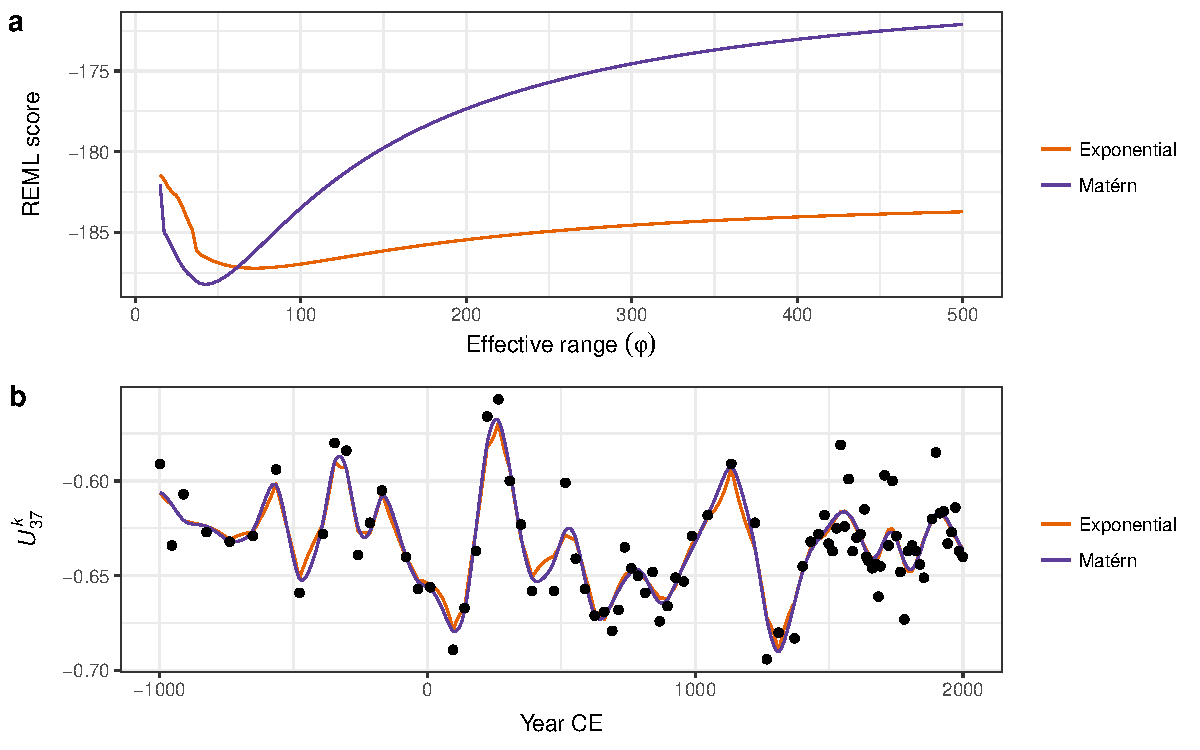
\includegraphics[width=0.8\linewidth]{supplementary-materials_files/figure-latex/gp-gam-detail-plot-1} \end{center}

Next we extract the minimum of the REML scores for the two correlation
functions and refit those models (we threw away all the models in the
\texttt{for\ ()} loop earlier to avoid storing lots of model objects).
Then we fit GAMs with Gaussian process smooths using the values of
\(\phi\) that produced the minimum REML scores, and predict using the
fitted models to visualize the trends.

\begin{Shaded}
\begin{Highlighting}[]
\NormalTok{## effective range minima from profile likelihood}
\NormalTok{effRange2 <-}\StringTok{ }\KeywordTok{with}\NormalTok{(}\KeywordTok{subset}\NormalTok{(reml.scr, cor ==}\StringTok{ "Matérn"}\NormalTok{), dseq[}\KeywordTok{which.min}\NormalTok{(reml)])}
\NormalTok{effRange3 <-}\StringTok{ }\KeywordTok{with}\NormalTok{(}\KeywordTok{subset}\NormalTok{(reml.scr, cor ==}\StringTok{ "Exponential"}\NormalTok{), dseq[}\KeywordTok{which.min}\NormalTok{(reml)])}

\NormalTok{## Refit these models: Matern}
\NormalTok{gp2 <-}\StringTok{ }\KeywordTok{gam}\NormalTok{(UK37 ~}\StringTok{ }\KeywordTok{s}\NormalTok{(Year, }\DataTypeTok{k =} \DecValTok{45}\NormalTok{, }\DataTypeTok{bs =} \StringTok{"gp"}\NormalTok{, }\DataTypeTok{m =} \KeywordTok{c}\NormalTok{(}\DecValTok{3}\NormalTok{, effRange2)),}
           \DataTypeTok{data =} \NormalTok{braya,}
           \DataTypeTok{method =} \StringTok{"REML"}\NormalTok{, }\DataTypeTok{weights =} \NormalTok{sampleInterval /}\StringTok{ }\KeywordTok{mean}\NormalTok{(sampleInterval))}
\NormalTok{## Refit these models: Power exponential}
\NormalTok{gp3 <-}\StringTok{ }\KeywordTok{gam}\NormalTok{(UK37 ~}\StringTok{ }\KeywordTok{s}\NormalTok{(Year, }\DataTypeTok{k =} \DecValTok{45}\NormalTok{, }\DataTypeTok{bs =} \StringTok{"gp"}\NormalTok{, }\DataTypeTok{m =} \KeywordTok{c}\NormalTok{(}\DecValTok{2}\NormalTok{, effRange3, }\DecValTok{1}\NormalTok{)),}
           \DataTypeTok{data =} \NormalTok{braya,}
           \DataTypeTok{method =} \StringTok{"REML"}\NormalTok{, }\DataTypeTok{weights =} \NormalTok{sampleInterval /}\StringTok{ }\KeywordTok{mean}\NormalTok{(sampleInterval))}

\NormalTok{## data to predict at}
\NormalTok{newd <-}\StringTok{ }\KeywordTok{with}\NormalTok{(braya, }\KeywordTok{data.frame}\NormalTok{(}\DataTypeTok{Year =} \KeywordTok{seq}\NormalTok{(}\KeywordTok{min}\NormalTok{(Year), }\KeywordTok{max}\NormalTok{(Year),}
                               \DataTypeTok{length.out =} \DecValTok{1000}\NormalTok{)))}
\NormalTok{## create predictions on response scale for both covariance functions}
\NormalTok{p.gp2 <-}\StringTok{ }\KeywordTok{transform}\NormalTok{(newd,}
                   \DataTypeTok{fitted =} \KeywordTok{predict}\NormalTok{(gp2, }\DataTypeTok{newdata =} \NormalTok{newd, }\DataTypeTok{type =} \StringTok{"response"}\NormalTok{),}
                   \DataTypeTok{effRange =} \KeywordTok{round}\NormalTok{(effRange2))}
\NormalTok{p.gp3 <-}\StringTok{ }\KeywordTok{transform}\NormalTok{(newd,}
                   \DataTypeTok{fitted =} \KeywordTok{predict}\NormalTok{(gp3, }\DataTypeTok{newdata =} \NormalTok{newd, }\DataTypeTok{type =} \StringTok{"response"}\NormalTok{),}
                   \DataTypeTok{effRange =} \KeywordTok{round}\NormalTok{(effRange3))}
\NormalTok{## joint the two sets of predictions together}
\NormalTok{pred <-}\StringTok{ }\KeywordTok{rbind}\NormalTok{(p.gp2, p.gp3)}
\NormalTok{## add some categorical variables for plotting}
\NormalTok{pred <-}\StringTok{ }\KeywordTok{transform}\NormalTok{(pred,}
                  \DataTypeTok{effRange =} \KeywordTok{factor}\NormalTok{(effRange),}
                  \DataTypeTok{cor =} \KeywordTok{rep}\NormalTok{(}\KeywordTok{c}\NormalTok{(}\StringTok{"Matérn"}\NormalTok{, }\StringTok{"Exponential"}\NormalTok{), }\DataTypeTok{each =} \KeywordTok{nrow}\NormalTok{(newd)))}
\end{Highlighting}
\end{Shaded}

The estimated Gaussian process trends are plotted using

\begin{Shaded}
\begin{Highlighting}[]
\NormalTok{gp.plt2 <-}\StringTok{ }\KeywordTok{ggplot}\NormalTok{(pred, }\KeywordTok{aes}\NormalTok{(}\DataTypeTok{x =} \NormalTok{Year, }\DataTypeTok{y =} \NormalTok{fitted, }\DataTypeTok{colour =} \NormalTok{cor)) +}
\StringTok{    }\KeywordTok{geom_line}\NormalTok{() +}\StringTok{ }\KeywordTok{theme}\NormalTok{(}\DataTypeTok{legend.position =} \StringTok{"right"}\NormalTok{) +}
\StringTok{    }\KeywordTok{geom_point}\NormalTok{(}\KeywordTok{aes}\NormalTok{(}\DataTypeTok{x =} \NormalTok{Year, }\DataTypeTok{y =} \NormalTok{UK37), }\DataTypeTok{data =} \NormalTok{braya, }\DataTypeTok{inherit.aes =} \OtherTok{FALSE}\NormalTok{) +}
\StringTok{    }\KeywordTok{scale_colour_manual}\NormalTok{(}\DataTypeTok{name =} \StringTok{""}\NormalTok{, }\DataTypeTok{values =} \KeywordTok{c}\NormalTok{(}\StringTok{"#e66101"}\NormalTok{,}\StringTok{"#5e3c99"}\NormalTok{)) +}
\StringTok{    }\KeywordTok{labs}\NormalTok{(}\DataTypeTok{y =} \NormalTok{braya_ylabel, }\DataTypeTok{x =} \StringTok{"Year CE"}\NormalTok{)}
\NormalTok{gp.plt2}
\end{Highlighting}
\end{Shaded}

\begin{center}\includegraphics[width=0.8\linewidth]{supplementary-materials_files/figure-latex/plot-both-gp-smooth-trends-1} \end{center}

whilst Figure 13 in the manuscript was prepared using

\begin{Shaded}
\begin{Highlighting}[]
\KeywordTok{plot_grid}\NormalTok{(proflik.plt, gp.plt2, }\DataTypeTok{ncol =} \DecValTok{1}\NormalTok{, }\DataTypeTok{labels =} \KeywordTok{c}\NormalTok{(}\StringTok{"a"}\NormalTok{,}\StringTok{"b"}\NormalTok{),}
          \DataTypeTok{align =} \StringTok{"hv"}\NormalTok{, }\DataTypeTok{axis =} \StringTok{"lr"}\NormalTok{)}
\end{Highlighting}
\end{Shaded}

\section{Adaptive smooths}\label{adaptive-smooths}

The adaptive smooth was fitted to the Braya-Sø data by adding
\texttt{bs\ =\ "ad"} to the \texttt{s()} term in the model formula. The
other aspects of the fit are as previously used for the other models,
REML smoothness selection and observational weights:

\begin{Shaded}
\begin{Highlighting}[]
\NormalTok{## Adaptive spline, weights as sampleInterval}
\NormalTok{mod_ad <-}\StringTok{ }\KeywordTok{gam}\NormalTok{(UK37 ~}\StringTok{ }\KeywordTok{s}\NormalTok{(Year, }\DataTypeTok{k =} \DecValTok{45}\NormalTok{, }\DataTypeTok{bs =} \StringTok{"ad"}\NormalTok{), }\DataTypeTok{data =} \NormalTok{braya,}
              \DataTypeTok{method =} \StringTok{"REML"}\NormalTok{,}
              \DataTypeTok{weights =} \NormalTok{sampleInterval /}\StringTok{ }\KeywordTok{mean}\NormalTok{(sampleInterval))}
\end{Highlighting}
\end{Shaded}

\section{Comparing trends}\label{comparing-trends}

For the model comparison I refitted all the models for consistency; the
code to fit each of the

\begin{enumerate}
\def\labelenumi{\arabic{enumi}.}
\tightlist
\item
  Thin plate regression spline (TPRS),
\item
  Gaussian process spline (Matérn correlation functions), and
\item
  Adaptive smoother
\end{enumerate}

is shown below.

\begin{Shaded}
\begin{Highlighting}[]
\NormalTok{## effective range parameter from profile-likelihood of Matern model}
\NormalTok{effRange <-}\StringTok{ }\NormalTok{effRange2}

\NormalTok{## TPRS, weights as sampleInterval}
\NormalTok{mod_tprs <-}\StringTok{ }\KeywordTok{gam}\NormalTok{(UK37 ~}\StringTok{ }\KeywordTok{s}\NormalTok{(Year, }\DataTypeTok{k =} \DecValTok{45}\NormalTok{, }\DataTypeTok{bs =} \StringTok{"tp"}\NormalTok{), }\DataTypeTok{data =} \NormalTok{braya,}
                \DataTypeTok{method =} \StringTok{"REML"}\NormalTok{,}
                \DataTypeTok{weights =} \NormalTok{sampleInterval /}\StringTok{ }\KeywordTok{mean}\NormalTok{(sampleInterval))}

\NormalTok{## Gaussian process, Matern, kappa = 1.5, weights as sampleInterval}
\NormalTok{mod_gp <-}\StringTok{ }\KeywordTok{gam}\NormalTok{(UK37 ~}\StringTok{ }\KeywordTok{s}\NormalTok{(Year, }\DataTypeTok{k =} \DecValTok{45}\NormalTok{, }\DataTypeTok{bs =} \StringTok{"gp"}\NormalTok{, }\DataTypeTok{m =} \KeywordTok{c}\NormalTok{(}\DecValTok{3}\NormalTok{, effRange)),}
              \DataTypeTok{data =} \NormalTok{braya,}
              \DataTypeTok{method =} \StringTok{"REML"}\NormalTok{,}
              \DataTypeTok{weights =} \NormalTok{sampleInterval /}\StringTok{ }\KeywordTok{mean}\NormalTok{(sampleInterval))}

\NormalTok{## Adaptive spline, weights as sampleInterval}
\NormalTok{mod_ad <-}\StringTok{ }\KeywordTok{gam}\NormalTok{(UK37 ~}\StringTok{ }\KeywordTok{s}\NormalTok{(Year, }\DataTypeTok{k =} \DecValTok{45}\NormalTok{, }\DataTypeTok{bs =} \StringTok{"ad"}\NormalTok{), }\DataTypeTok{data =} \NormalTok{braya,}
              \DataTypeTok{method =} \StringTok{"REML"}\NormalTok{,}
              \DataTypeTok{weights =} \NormalTok{sampleInterval /}\StringTok{ }\KeywordTok{mean}\NormalTok{(sampleInterval))}
\end{Highlighting}
\end{Shaded}

I wrote a small function to predict from each model over the range of
\texttt{Year} and return the data in tidy format for plotting.

\begin{Shaded}
\begin{Highlighting}[]
\NormalTok{## wrap this in a function that will return all the plots & derived objects}
\NormalTok{processGAM <-}\StringTok{ }\NormalTok{function(mod) \{}
    \NormalTok{## Predict from model}
    \NormalTok{N <-}\StringTok{ }\DecValTok{500}
    \NormalTok{newYear <-}\StringTok{ }\KeywordTok{with}\NormalTok{(braya,}
                    \KeywordTok{data.frame}\NormalTok{(}\DataTypeTok{Year =} \KeywordTok{seq}\NormalTok{(}\KeywordTok{min}\NormalTok{(Year), }\KeywordTok{max}\NormalTok{(Year),}
                                          \DataTypeTok{length.out =} \NormalTok{N)))}
    \NormalTok{newYear <-}\StringTok{ }\KeywordTok{cbind}\NormalTok{(newYear,}
                     \KeywordTok{data.frame}\NormalTok{(}\KeywordTok{predict}\NormalTok{(mod, newYear, }\DataTypeTok{se.fit =} \OtherTok{TRUE}\NormalTok{)))}
    
    \NormalTok{out <-}\StringTok{ }\KeywordTok{list}\NormalTok{(}\DataTypeTok{objects =} \NormalTok{newYear)}
    \NormalTok{out}
\NormalTok{\}}

\NormalTok{plts_gp   <-}\StringTok{ }\KeywordTok{processGAM}\NormalTok{(}\DataTypeTok{mod =} \NormalTok{mod_gp) }\CommentTok{# Gaussian process smooth with weights}
\NormalTok{plts_ad   <-}\StringTok{ }\KeywordTok{processGAM}\NormalTok{(}\DataTypeTok{mod =} \NormalTok{mod_ad) }\CommentTok{# Adaptive smooth with weights}
\NormalTok{plts_tprs <-}\StringTok{ }\KeywordTok{processGAM}\NormalTok{(}\DataTypeTok{mod =} \NormalTok{mod_tprs) }\CommentTok{# TPRS with weights}

\NormalTok{pltData <-}\StringTok{ }\KeywordTok{do.call}\NormalTok{(}\StringTok{"rbind"}\NormalTok{, }\KeywordTok{lapply}\NormalTok{(}\KeywordTok{list}\NormalTok{(plts_gp, plts_ad, plts_tprs),}
                                   \StringTok{`}\DataTypeTok{[[}\StringTok{`}\NormalTok{, }\StringTok{"objects"}\NormalTok{))}
\NormalTok{pltData <-}\StringTok{ }\KeywordTok{transform}\NormalTok{(pltData,}
                     \DataTypeTok{Model =} \KeywordTok{rep}\NormalTok{(}\KeywordTok{c}\NormalTok{(}\StringTok{"GP"}\NormalTok{, }\StringTok{"Adaptive"}\NormalTok{, }\StringTok{"TPRS"}\NormalTok{),}
                                 \DataTypeTok{each =} \KeywordTok{nrow}\NormalTok{(plts_gp$objects)))}

\NormalTok{allFits <-}\StringTok{ }\KeywordTok{ggplot}\NormalTok{(pltData, }\KeywordTok{aes}\NormalTok{(}\DataTypeTok{x =} \NormalTok{Year, }\DataTypeTok{y =} \NormalTok{fit)) +}
\StringTok{    }\KeywordTok{geom_point}\NormalTok{(}\KeywordTok{aes}\NormalTok{(}\DataTypeTok{x =} \NormalTok{Year, }\DataTypeTok{y =} \NormalTok{UK37), }\DataTypeTok{data =} \NormalTok{braya) +}
\StringTok{    }\KeywordTok{geom_line}\NormalTok{(}\KeywordTok{aes}\NormalTok{(}\DataTypeTok{colour =} \NormalTok{Model)) +}\StringTok{ }\KeywordTok{labs}\NormalTok{(}\DataTypeTok{y =} \NormalTok{braya_ylabel, }\DataTypeTok{x =} \StringTok{"Year"}\NormalTok{) +}
\StringTok{    }\KeywordTok{theme}\NormalTok{(}\DataTypeTok{legend.position =} \StringTok{"right"}\NormalTok{) +}
\StringTok{    }\KeywordTok{scale_colour_manual}\NormalTok{(}\DataTypeTok{name =} \StringTok{""}\NormalTok{,}
                        \DataTypeTok{values =} \KeywordTok{c}\NormalTok{(}\StringTok{"#e66101"}\NormalTok{, }\StringTok{"#fdb863"}\NormalTok{, }\StringTok{"#5e3c99"}\NormalTok{))}
\NormalTok{allFits}
\end{Highlighting}
\end{Shaded}

\begin{center}\includegraphics[width=0.8\linewidth]{supplementary-materials_files/figure-latex/process-models-1} \end{center}

The plot produced reproduces Figure 14 in the manuscript.

\section{Accounting for age-model
uncertainty}\label{accounting-for-age-model-uncertainty}

The manuscript proposed to simulate from the posterior distribution of
the fitted age model as a way to account for age-model uncertainty. The
first step in the process is to fit the age model from which to simulate
new age models. This was done using the \emph{scam} package for a
\emph{shape-constrained GAM}, with the age-model spline constrained to
be monotonic decreasing (\texttt{bs\ =\ "mpd"}).

To make this section self-contained, I refitted the Small Water GAM plus
CAR(1) model. Because we will be sampling ages for each observation from
the posterior of the age-model GAM, the oldest sample will will be
somewhat younger than the expected value from the model in some samples.
This will cause problems when we come to simulate from the GAMs fitted
to the resampled age-models as each GAM will cover a slightly different
range of time. To avoid this problem I fix the knots at the extremes of
the observed values of \texttt{Year} and spread the remaining 12 knots
evenly inbetween. The knot locations are stored in the vector
\texttt{knots}, which is passed to the argument \texttt{knots} when
fitting the GAM

\begin{Shaded}
\begin{Highlighting}[]
\NormalTok{knots <-}\StringTok{ }\KeywordTok{with}\NormalTok{(small, }\KeywordTok{list}\NormalTok{(}\DataTypeTok{Year =} \KeywordTok{seq}\NormalTok{(}\KeywordTok{min}\NormalTok{(Year), }\KeywordTok{max}\NormalTok{(Year), }\DataTypeTok{length =} \DecValTok{14}\NormalTok{)))}
\NormalTok{mod <-}\StringTok{ }\KeywordTok{gamm}\NormalTok{(d15N ~}\StringTok{ }\KeywordTok{s}\NormalTok{(Year, }\DataTypeTok{k =} \DecValTok{15}\NormalTok{), }\DataTypeTok{data =} \NormalTok{small, }\DataTypeTok{method =} \StringTok{"REML"}\NormalTok{,}
            \DataTypeTok{correlation =} \KeywordTok{corCAR1}\NormalTok{(}\DataTypeTok{form =} \NormalTok{~}\StringTok{ }\NormalTok{Year),}
            \DataTypeTok{knots =} \NormalTok{knots)}
\end{Highlighting}
\end{Shaded}

Setting the knots like this doesn't change the model estimated above;
I'm only repeating what happens internally if you don't supply
\texttt{knots}. However, later we will need to specify this set of knots
explicitly when accounting for age model uncertainty.

Next we load the \textsuperscript{210}Pb dating results for the dated
core sections.

\begin{Shaded}
\begin{Highlighting}[]
\NormalTok{swAge <-}\StringTok{ }\KeywordTok{read.csv}\NormalTok{(}\StringTok{"./data/small-water/small1-dating.csv"}\NormalTok{)}
\end{Highlighting}
\end{Shaded}

before fitting the shape-constrained GAM. Currently, \emph{scam} can
only fit models using GCV smoothness selection. I used the
\texttt{gamma} argument here to add a larger penalty for more-complex
models. Each effective degree of freedom used by the spline is counted
as 1.4 degrees of freedom in the GCV score.

\begin{Shaded}
\begin{Highlighting}[]
\NormalTok{## monotonic spline age-depth model}
\NormalTok{swAge$Error[}\DecValTok{1}\NormalTok{] <-}\StringTok{ }\FloatTok{1.1}
\NormalTok{swAgeMod <-}\StringTok{ }\KeywordTok{scam}\NormalTok{(Date ~}\StringTok{ }\KeywordTok{s}\NormalTok{(Depth, }\DataTypeTok{k =} \DecValTok{5}\NormalTok{, }\DataTypeTok{bs =} \StringTok{"mpd"}\NormalTok{), }\DataTypeTok{data =} \NormalTok{swAge,}
                 \DataTypeTok{weights =} \DecValTok{1} \NormalTok{/}\StringTok{ }\NormalTok{swAge$Error, }\DataTypeTok{gamma =} \FloatTok{1.4}\NormalTok{)}
\end{Highlighting}
\end{Shaded}

Note that I added a small amount of error to the surface sample age as
the model cannot be fitted if an observation has \texttt{0} weight.

Next, predict from the estimated age model, and draw 25 samples from the
posterior distribution using \texttt{simulate()}. The results are tidied
into a format suitable for further processing and plotting. Note that
the posterior samples here are only used for plotting.

\begin{Shaded}
\begin{Highlighting}[]
\NormalTok{## predict from the age model for a smooth set of points in `Depth`}
\NormalTok{newAge <-}\StringTok{ }\KeywordTok{with}\NormalTok{(swAge, }\KeywordTok{data.frame}\NormalTok{(}\DataTypeTok{Depth =} \KeywordTok{seq}\NormalTok{(}\KeywordTok{min}\NormalTok{(Depth), }\KeywordTok{max}\NormalTok{(Depth),}
                                             \DataTypeTok{length.out =} \DecValTok{200}\NormalTok{)))}
\NormalTok{newAge <-}\StringTok{ }\KeywordTok{transform}\NormalTok{(newAge,}
                    \DataTypeTok{fitted =} \KeywordTok{predict}\NormalTok{(swAgeMod, }\DataTypeTok{newdata =} \NormalTok{newAge, }
                                     \DataTypeTok{type =} \StringTok{"response"}\NormalTok{))}
\NormalTok{newSims <-}\StringTok{ }\KeywordTok{as.data.frame}\NormalTok{(}\KeywordTok{simulate}\NormalTok{(swAgeMod, }\DataTypeTok{nsim =} \DecValTok{25}\NormalTok{, }\DataTypeTok{newdata =} \NormalTok{newAge))}
\NormalTok{newSims <-}\StringTok{ }\KeywordTok{cbind}\NormalTok{(}\DataTypeTok{Depth =} \NormalTok{newAge$Depth, newSims)}
\NormalTok{newSims <-}\StringTok{ }\KeywordTok{gather}\NormalTok{(newSims, Simulation, Age, -Depth)}
\end{Highlighting}
\end{Shaded}

In the next code chunk, I draw 100 samples from the posterior
distribution of the age model, but notice that I pass in the
\texttt{small} data to \texttt{newdata} in the call to
\texttt{simulate()} as the locations I want new age estimates for are
the depths for which we have δ\textsuperscript{15}N values. A small
function (\texttt{fitSWModels}) is written to prepare each simulation
for fitting and then actually fit the GAM plus CAR(1) model using the
updated age information.

\begin{Shaded}
\begin{Highlighting}[]
\NormalTok{## simulate from age model; each column is a simulation}
\NormalTok{ageSims <-}\StringTok{ }\KeywordTok{simulate}\NormalTok{(swAgeMod, }\DataTypeTok{nsim =} \DecValTok{100}\NormalTok{, }\DataTypeTok{newdata =} \NormalTok{small, }\DataTypeTok{seed =} \DecValTok{42}\NormalTok{)}
\NormalTok{ageSims <-}\StringTok{ }\KeywordTok{as.data.frame}\NormalTok{(ageSims)}

\NormalTok{fitSWModels <-}\StringTok{ }\NormalTok{function(x, y, knots) \{}
    \NormalTok{dat <-}\StringTok{ }\KeywordTok{data.frame}\NormalTok{(}\DataTypeTok{d15N =} \NormalTok{y, }\DataTypeTok{Year =} \NormalTok{x)}
    \NormalTok{m <-}\StringTok{ }\KeywordTok{gamm}\NormalTok{(d15N ~}\StringTok{ }\KeywordTok{s}\NormalTok{(Year, }\DataTypeTok{k =} \DecValTok{15}\NormalTok{), }\DataTypeTok{data =} \NormalTok{dat, }\DataTypeTok{method =} \StringTok{"REML"}\NormalTok{,}
              \DataTypeTok{correlation =} \KeywordTok{corCAR1}\NormalTok{(}\DataTypeTok{form =} \NormalTok{~}\StringTok{ }\NormalTok{Year), }\DataTypeTok{knots =} \NormalTok{knots)}
\NormalTok{\}}

\NormalTok{## generate new trends using draws from age-model posterior}
\NormalTok{simTrendMods <-}\StringTok{ }\KeywordTok{lapply}\NormalTok{(ageSims, fitSWModels, }\DataTypeTok{y =} \NormalTok{small$d15N, }\DataTypeTok{knots =} \NormalTok{knots)}


\NormalTok{## function wrapper to predict new trends at locations over the}
\NormalTok{## range of `Year`}
\NormalTok{predSWModels <-}\StringTok{ }\NormalTok{function(mod, newdata) \{}
    \KeywordTok{predict}\NormalTok{(mod$gam, }\DataTypeTok{newdata =} \NormalTok{newdata, }\DataTypeTok{type =} \StringTok{"response"}\NormalTok{)}
\NormalTok{\}}

\NormalTok{## predict from fitted model to produce a smooth trend for each posterior}
\NormalTok{## sample}
\NormalTok{simTrends <-}\StringTok{ }\KeywordTok{lapply}\NormalTok{(simTrendMods, predSWModels, }\DataTypeTok{newdata =} \NormalTok{newYear)}

\NormalTok{## arrange in a tidy format form plottings}
\NormalTok{simTrends <-}\StringTok{ }\KeywordTok{data.frame}\NormalTok{(}\DataTypeTok{Year  =} \KeywordTok{with}\NormalTok{(newYear, }\KeywordTok{rep}\NormalTok{(Year, }\KeywordTok{length}\NormalTok{(simTrends))),}
                        \DataTypeTok{Trend =} \KeywordTok{unlist}\NormalTok{(simTrends),}
                        \DataTypeTok{Group =} \KeywordTok{rep}\NormalTok{(}\KeywordTok{seq_along}\NormalTok{(simTrends),}
                                    \DataTypeTok{times =} \KeywordTok{lengths}\NormalTok{(simTrends)))}
\end{Highlighting}
\end{Shaded}

The next chunk does the final step in the process. For each of the
models we just fitted, we simulate 50 draws from the model posterior
distribution. We start with a wrapper function around the
\texttt{simulate()} code we want to run on each model, then do the
actual posterior draws for each model using \texttt{lapply()}. The final
step just arranges data for plotting.

\begin{Shaded}
\begin{Highlighting}[]
\NormalTok{## wrapper to simulate from a fitted GAM with the required arguments}
\NormalTok{simulateSWModels <-}\StringTok{ }\NormalTok{function(mod, newdata, nsim, }\DataTypeTok{seed =} \DecValTok{42}\NormalTok{) \{}
    \NormalTok{sims <-}\StringTok{ }\KeywordTok{simulate}\NormalTok{(mod, }\DataTypeTok{nsim =} \NormalTok{nsim, }\DataTypeTok{newdata =} \NormalTok{newdata, }\DataTypeTok{seed =} \NormalTok{seed)}
    \KeywordTok{as.vector}\NormalTok{(sims)}
\NormalTok{\}}

\NormalTok{## now do the posterior simulation}
\NormalTok{NSIM <-}\StringTok{ }\DecValTok{50}     \CommentTok{# number of posterior samples *per* model}
\NormalTok{simSimulate <-}\StringTok{ }\KeywordTok{lapply}\NormalTok{(simTrendMods, simulateSWModels, }\DataTypeTok{newdata =} \NormalTok{newYear,}
                      \DataTypeTok{nsim =} \NormalTok{NSIM, }\DataTypeTok{seed =} \DecValTok{42}\NormalTok{)}

\NormalTok{## arrange in a tidy format}
\NormalTok{simSimulate <-}
\StringTok{  }\KeywordTok{data.frame}\NormalTok{(}\DataTypeTok{Year  =} \KeywordTok{with}\NormalTok{(newYear,}
                          \KeywordTok{rep}\NormalTok{(Year, }\DataTypeTok{times =} \NormalTok{NSIM *}\StringTok{ }\KeywordTok{length}\NormalTok{(simSimulate))),}
             \DataTypeTok{Trend =} \KeywordTok{unlist}\NormalTok{(simSimulate),}
             \DataTypeTok{Group =} \KeywordTok{rep}\NormalTok{(}\KeywordTok{seq_len}\NormalTok{(NSIM *}\StringTok{ }\KeywordTok{length}\NormalTok{(simSimulate)),}
                         \DataTypeTok{each =} \KeywordTok{nrow}\NormalTok{(newYear)))}
\end{Highlighting}
\end{Shaded}

Each of the steps is visualized using the plot code shown below.

\begin{Shaded}
\begin{Highlighting}[]
\NormalTok{## plot the estimated age model ad posterior simulations from it}
\NormalTok{plt1 <-}\StringTok{ }\KeywordTok{ggplot}\NormalTok{(swAge, }\KeywordTok{aes}\NormalTok{(}\DataTypeTok{y =} \NormalTok{Date, }\DataTypeTok{x =} \NormalTok{Depth)) +}
\StringTok{    }\KeywordTok{geom_line}\NormalTok{(}\DataTypeTok{data =} \NormalTok{newSims,}
              \DataTypeTok{mapping =} \KeywordTok{aes}\NormalTok{(}\DataTypeTok{y =} \NormalTok{Age, }\DataTypeTok{x =} \NormalTok{Depth, }\DataTypeTok{group =} \NormalTok{Simulation),}
              \DataTypeTok{alpha =} \DecValTok{1}\NormalTok{, }\DataTypeTok{colour =} \StringTok{"grey80"}\NormalTok{) +}
\StringTok{    }\KeywordTok{geom_line}\NormalTok{(}\DataTypeTok{data =} \NormalTok{newAge, }\DataTypeTok{mapping =} \KeywordTok{aes}\NormalTok{(}\DataTypeTok{y =} \NormalTok{fitted, }\DataTypeTok{x =} \NormalTok{Depth)) +}
\StringTok{    }\KeywordTok{geom_point}\NormalTok{(}\DataTypeTok{size =} \FloatTok{1.5}\NormalTok{, }\DataTypeTok{colour =} \StringTok{"red"}\NormalTok{) +}
\StringTok{    }\KeywordTok{geom_errorbar}\NormalTok{(}\KeywordTok{aes}\NormalTok{(}\DataTypeTok{ymin =} \NormalTok{Date -}\StringTok{ }\NormalTok{Error, }\DataTypeTok{ymax =} \NormalTok{Date +}\StringTok{ }\NormalTok{Error, }\DataTypeTok{width =} \DecValTok{0}\NormalTok{),}
                  \DataTypeTok{colour =} \StringTok{"red"}\NormalTok{) +}
\StringTok{    }\KeywordTok{labs}\NormalTok{(}\DataTypeTok{y =} \StringTok{"Year CE"}\NormalTok{, }\DataTypeTok{x =} \StringTok{"Depth (cm)"}\NormalTok{)}

\NormalTok{## plot the simulated trends showing the effect of age-model uncertainty}
\NormalTok{plt2 <-}\StringTok{ }\KeywordTok{ggplot}\NormalTok{(simTrends, }\KeywordTok{aes}\NormalTok{(}\DataTypeTok{x =} \NormalTok{Year, }\DataTypeTok{y =} \NormalTok{Trend, }\DataTypeTok{group =} \NormalTok{Group)) +}
\StringTok{    }\KeywordTok{geom_line}\NormalTok{(}\DataTypeTok{alpha =} \FloatTok{0.1}\NormalTok{, }\DataTypeTok{colour =} \StringTok{"grey80"}\NormalTok{) +}
\StringTok{    }\KeywordTok{geom_line}\NormalTok{(}\DataTypeTok{data =} \NormalTok{newYear,}
              \DataTypeTok{mapping =} \KeywordTok{aes}\NormalTok{(}\DataTypeTok{x =} \NormalTok{Year, }\DataTypeTok{y =} \NormalTok{fit), }\DataTypeTok{inherit.aes =} \OtherTok{FALSE}\NormalTok{) +}
\StringTok{    }\KeywordTok{geom_point}\NormalTok{(}\DataTypeTok{data =} \NormalTok{small,}
               \DataTypeTok{mapping =} \KeywordTok{aes}\NormalTok{(}\DataTypeTok{x =} \NormalTok{Year, }\DataTypeTok{y =} \NormalTok{d15N),}
               \DataTypeTok{inherit.aes =} \OtherTok{FALSE}\NormalTok{, }\DataTypeTok{size =} \FloatTok{0.7}\NormalTok{) +}
\StringTok{    }\KeywordTok{labs}\NormalTok{(}\DataTypeTok{x =} \StringTok{"Year"}\NormalTok{, }\DataTypeTok{y =} \NormalTok{d15n_label)}

\NormalTok{## plot simulated trends showing the effect of age-model uncertainty and}
\NormalTok{## the effect of uncertainty in the estimated trend itself}
\NormalTok{plt3 <-}\StringTok{ }\KeywordTok{ggplot}\NormalTok{(simSimulate, }\KeywordTok{aes}\NormalTok{(}\DataTypeTok{x =} \NormalTok{Year, }\DataTypeTok{y =} \NormalTok{Trend, }\DataTypeTok{group =} \NormalTok{Group)) +}
\StringTok{    }\KeywordTok{geom_line}\NormalTok{(}\DataTypeTok{alpha =} \FloatTok{0.2}\NormalTok{, }\DataTypeTok{colour =} \StringTok{"grey80"}\NormalTok{) +}
\StringTok{    }\KeywordTok{geom_point}\NormalTok{(}\DataTypeTok{data =} \NormalTok{small,}
               \DataTypeTok{mapping =} \KeywordTok{aes}\NormalTok{(}\DataTypeTok{x =} \NormalTok{Year, }\DataTypeTok{y =} \NormalTok{d15N),}
               \DataTypeTok{inherit.aes =} \OtherTok{FALSE}\NormalTok{,}
               \DataTypeTok{size =} \FloatTok{0.7}\NormalTok{) +}
\StringTok{    }\KeywordTok{geom_line}\NormalTok{(}\DataTypeTok{data =} \NormalTok{newYear,}
              \DataTypeTok{mapping =} \KeywordTok{aes}\NormalTok{(}\DataTypeTok{x =} \NormalTok{Year, }\DataTypeTok{y =} \NormalTok{fit),}
              \DataTypeTok{inherit.aes =} \OtherTok{FALSE}\NormalTok{) +}
\StringTok{    }\KeywordTok{labs}\NormalTok{(}\DataTypeTok{x =} \StringTok{"Year"}\NormalTok{, }\DataTypeTok{y =} \NormalTok{d15n_label)}

\NormalTok{## align all plots vertically}
\NormalTok{plots <-}\StringTok{ }\KeywordTok{align_plots}\NormalTok{(plt1, plt2, plt3, }\DataTypeTok{align =} \StringTok{'v'}\NormalTok{, }\DataTypeTok{axis =} \StringTok{'l'}\NormalTok{)}


\NormalTok{## create the two rows of figures, from `plots`}
\NormalTok{top_row <-}\StringTok{ }\KeywordTok{plot_grid}\NormalTok{(plots[[}\DecValTok{1}\NormalTok{]], }\OtherTok{NULL}\NormalTok{, }\DataTypeTok{ncol =} \DecValTok{2}\NormalTok{, }\DataTypeTok{labels =} \StringTok{"a"}\NormalTok{)}
\NormalTok{bot_row <-}\StringTok{ }\KeywordTok{plot_grid}\NormalTok{(plots[[}\DecValTok{2}\NormalTok{]], plots[[}\DecValTok{3}\NormalTok{]], }\DataTypeTok{ncol =} \DecValTok{1}\NormalTok{, }\DataTypeTok{labels =} \KeywordTok{c}\NormalTok{(}\StringTok{"b"}\NormalTok{, }\StringTok{"c"}\NormalTok{))}

\NormalTok{## combine the two rows, top row has 1 plot row, bottom row has 2, hence}
\NormalTok{## the rel_heights to even this out}
\KeywordTok{plot_grid}\NormalTok{(top_row, bot_row, }\DataTypeTok{ncol =} \DecValTok{1}\NormalTok{, }\DataTypeTok{rel_heights =} \KeywordTok{c}\NormalTok{(}\FloatTok{0.5}\NormalTok{, }\DecValTok{1}\NormalTok{))}
\end{Highlighting}
\end{Shaded}

\begin{center}\includegraphics[width=0.8\linewidth]{supplementary-materials_files/figure-latex/small-scam-fit-plots-1} \end{center}

This reproduces Figure 15 from the manuscript.

\section{Session information}\label{session-information}

\begin{Shaded}
\begin{Highlighting}[]
\NormalTok{devtools::}\KeywordTok{session_info}\NormalTok{()}
\end{Highlighting}
\end{Shaded}

\begin{verbatim}
#> Session info -------------------------------------------------------------
\end{verbatim}

\begin{verbatim}
#>  setting  value                                      
#>  version  R version 3.4.3 Patched (2018-01-16 r74126)
#>  system   x86_64, linux-gnu                          
#>  ui       X11                                        
#>  language (EN)                                       
#>  collate  en_CA.UTF-8                                
#>  tz       America/Regina                             
#>  date     2018-08-16
\end{verbatim}

\begin{verbatim}
#> Packages -----------------------------------------------------------------
\end{verbatim}

\begin{verbatim}
#>  package    * version date       source        
#>  assertthat   0.2.0   2017-04-11 CRAN (R 3.4.3)
#>  backports    1.1.2   2017-12-13 CRAN (R 3.4.3)
#>  base       * 3.4.3   2018-01-16 local         
#>  bindr        0.1.1   2018-03-13 CRAN (R 3.4.3)
#>  bindrcpp     0.2.2   2018-03-29 CRAN (R 3.4.3)
#>  codetools    0.2-15  2016-10-05 CRAN (R 3.4.3)
#>  colorspace   1.3-2   2016-12-14 CRAN (R 3.4.3)
#>  compiler     3.4.3   2018-01-16 local         
#>  cowplot    * 0.9.3   2018-07-15 CRAN (R 3.4.3)
#>  crayon       1.3.4   2017-09-16 CRAN (R 3.4.3)
#>  datasets   * 3.4.3   2018-01-16 local         
#>  devtools     1.13.6  2018-06-27 CRAN (R 3.4.3)
#>  digest       0.6.15  2018-01-28 CRAN (R 3.4.3)
#>  dplyr        0.7.6   2018-06-29 CRAN (R 3.4.3)
#>  evaluate     0.11    2018-07-17 CRAN (R 3.4.3)
#>  ggplot2    * 3.0.0   2018-07-03 CRAN (R 3.4.3)
#>  glue         1.3.0   2018-07-17 CRAN (R 3.4.3)
#>  graphics   * 3.4.3   2018-01-16 local         
#>  gratia     * 0.0-6   2018-08-16 local         
#>  grDevices  * 3.4.3   2018-01-16 local         
#>  grid         3.4.3   2018-01-16 local         
#>  gtable       0.2.0   2016-02-26 CRAN (R 3.4.3)
#>  htmltools    0.3.6   2017-04-28 CRAN (R 3.4.3)
#>  knitr        1.20    2018-02-20 CRAN (R 3.4.3)
#>  labeling     0.3     2014-08-23 CRAN (R 3.4.3)
#>  lattice      0.20-35 2017-03-25 CRAN (R 3.4.3)
#>  lazyeval     0.2.1   2017-10-29 CRAN (R 3.4.3)
#>  magrittr     1.5     2014-11-22 CRAN (R 3.4.3)
#>  MASS         7.3-50  2018-04-30 CRAN (R 3.4.3)
#>  Matrix       1.2-14  2018-04-09 CRAN (R 3.4.3)
#>  memoise      1.1.0   2017-04-21 CRAN (R 3.4.3)
#>  methods      3.4.3   2018-01-16 local         
#>  mgcv       * 1.8-24  2018-06-18 CRAN (R 3.4.3)
#>  munsell      0.5.0   2018-06-12 CRAN (R 3.4.3)
#>  nlme       * 3.1-137 2018-04-07 CRAN (R 3.4.3)
#>  pillar       1.3.0   2018-07-14 CRAN (R 3.4.3)
#>  pkgconfig    2.0.1   2017-03-21 CRAN (R 3.4.3)
#>  plyr         1.8.4   2016-06-08 CRAN (R 3.4.3)
#>  purrr        0.2.5   2018-05-29 CRAN (R 3.4.3)
#>  R6           2.2.2   2017-06-17 CRAN (R 3.4.3)
#>  Rcpp         0.12.18 2018-07-23 CRAN (R 3.4.3)
#>  rlang        0.2.1   2018-05-30 CRAN (R 3.4.3)
#>  rmarkdown  * 1.10    2018-06-11 CRAN (R 3.4.3)
#>  rprojroot    1.3-2   2018-01-03 CRAN (R 3.4.3)
#>  scales       0.5.0   2017-08-24 CRAN (R 3.4.3)
#>  scam       * 1.2-2   2017-09-24 CRAN (R 3.4.3)
#>  splines      3.4.3   2018-01-16 local         
#>  stats      * 3.4.3   2018-01-16 local         
#>  stringi      1.2.4   2018-07-20 CRAN (R 3.4.3)
#>  stringr      1.3.1   2018-05-10 CRAN (R 3.4.3)
#>  tibble       1.4.2   2018-01-22 CRAN (R 3.4.3)
#>  tidyr      * 0.8.1   2018-05-18 CRAN (R 3.4.3)
#>  tidyselect   0.2.4   2018-02-26 CRAN (R 3.4.3)
#>  tools        3.4.3   2018-01-16 local         
#>  utils      * 3.4.3   2018-01-16 local         
#>  withr        2.1.2   2018-03-15 CRAN (R 3.4.3)
#>  yaml         2.2.0   2018-07-25 CRAN (R 3.4.3)
\end{verbatim}


\end{document}
